%%%%%%%%%%%%%%%%%%%%%%%%%%%%%%%%%%%%%%%%%
% Short Sectioned Assignment LaTeX Template Version 1.0 (5/5/12)
% This template has been downloaded from: http://www.LaTeXTemplates.com
% Original author:  Frits Wenneker (http://www.howtotex.com)
% License: CC BY-NC-SA 3.0 (http://creativecommons.org/licenses/by-nc-sa/3.0/)
%%%%%%%%%%%%%%%%%%%%%%%%%%%%%%%%%%%%%%%%%

%----------------------------------------------------------------------------------------
%	PACKAGES AND OTHER DOCUMENT CONFIGURATIONS
%----------------------------------------------------------------------------------------

\documentclass[paper=a4, fontsize=11pt]{scrartcl} % A4 paper and 11pt font size

% ---- Entrada y salida de texto -----

\usepackage[T1]{fontenc} % Use 8-bit encoding that has 256 glyphs
\usepackage[utf8]{inputenc}
%\usepackage{fourier} % Use the Adobe Utopia font for the document - comment this line to return to the LaTeX default

% ---- Idioma --------

\usepackage[spanish, es-tabla]{babel} % Selecciona el español para palabras introducidas automáticamente, p.ej. "septiembre" en la fecha y especifica que se use la palabra Tabla en vez de Cuadro

% ---- Otros paquetes ----

\usepackage{url} % ,href} %para incluir URLs e hipervínculos dentro del texto (aunque hay que instalar href)
\usepackage{hyperref}
\hypersetup{
	colorlinks=true,
	linkcolor=black,
	urlcolor=black,
	citecolor=black,
}
\usepackage{amsmath,amsfonts,amsthm} % Math packages
%\usepackage{graphics,graphicx, floatrow} %para incluir imágenes y notas en las imágenes
\usepackage{graphics,graphicx, float} %para incluir imágenes y colocarlas

% Para hacer tablas comlejas
%\usepackage{multirow}
%\usepackage{threeparttable}

%\usepackage{sectsty} % Allows customizing section commands
%\allsectionsfont{\centering \normalfont\scshape} % Make all sections centered, the default font and small caps

\usepackage{fancyhdr} % Custom headers and footers
\pagestyle{fancyplain} % Makes all pages in the document conform to the custom headers and footers
\fancyhead{} % No page header - if you want one, create it in the same way as the footers below
\fancyfoot[L]{} % Empty left footer
\fancyfoot[C]{} % Empty center footer
\fancyfoot[R]{\thepage} % Page numbering for right footer
\renewcommand{\headrulewidth}{0pt} % Remove header underlines
\renewcommand{\footrulewidth}{0pt} % Remove footer underlines
\setlength{\headheight}{13.6pt} % Customize the height of the header

\numberwithin{equation}{section} % Number equations within sections (i.e. 1.1, 1.2, 2.1, 2.2 instead of 1, 2, 3, 4)
\numberwithin{figure}{section} % Number figures within sections (i.e. 1.1, 1.2, 2.1, 2.2 instead of 1, 2, 3, 4)
\numberwithin{table}{section} % Number tables within sections (i.e. 1.1, 1.2, 2.1, 2.2 instead of 1, 2, 3, 4)

\setlength\parindent{0pt} % Removes all indentation from paragraphs - comment this line for an assignment with lots of text

\newcommand{\horrule}[1]{\rule{\linewidth}{#1}} % Create horizontal rule command with 1 argument of height
\usepackage{booktabs}

\usepackage{listings}
\lstdefinelanguage
[x64]{Assembler}     % add a "x64" dialect of Assembler
[x86masm]{Assembler} % based on the "x86masm" dialect
{morekeywords={CDQE,CQO,CMPSQ,CMPXCHG16B,JRCXZ,LODSQ,MOVSXD, %
		POPFQ,PUSHFQ,SCASQ,STOSQ,IRETQ,RDTSCP,SWAPGS, %
		rax,rdx,rcx,rbx,rsi,rdi,rsp,rbp, %
		r8,r8d,r8w,r8b,r9,r9d,r9w,r9b, %
		r10,r10d,r10w,r10b,r11,r11d,r11w,r11b, %
		r12,r12d,r12w,r12b,r13,r13d,r13w,r13b, %
		r14,r14d,r14w,r14b,r15,r15d,r15w,r15b}} % etc.
\usepackage{color}
\usepackage{xcolor}
\lstdefinestyle{customc}{
	belowcaptionskip=1\baselineskip,
	breaklines=true,
	frame=L,
	xleftmargin=\parindent,
	language=C,
	showstringspaces=false,
	basicstyle=\footnotesize\ttfamily,
	keywordstyle=\bfseries\color{green!40!black},
	commentstyle=\itshape\color{purple!40!black},
	identifierstyle=\color{blue},
	stringstyle=\color{orange},
}

\lstset{escapechar=@,style=customc}
\usepackage{afterpage}


\setcounter{secnumdepth}{5}

\DeclareNewSectionCommand[
	style=section,
	counterwithin=subsubsection,
	afterskip=1.5ex plus .2ex,
	beforeskip=3.25ex plus 1ex minus .2ex,
	afterindent=false,
	level=\paragraphnumdepth,
	tocindent=10em,
	tocnumwidth=5em
]{subsubsubsection}

\setcounter{secnumdepth}{\subsubsubsectionnumdepth}
\setcounter{tocdepth}{\subparagraphtocdepth}

\RedeclareSectionCommands[
	level=\numexpr\subsubsubsectionnumdepth+1\relax,
	toclevel=\numexpr\subsubsubsectiontocdepth+1\relax,
	increaselevel
]{paragraph,subparagraph}

\RedeclareSectionCommand[
	counterwithin=subsubsubsection,
	tocindent=12em,
	tocnumwidth=6em
]{paragraph}

\RedeclareSectionCommand[
	tocindent=14em,
	tocnumwidth=7em
]{subparagraph}
\usepackage{url}

\title{	
	\normalfont \normalsize
	\begin{figure}[htb]
		\centering
		
\includegraphics[width=0.25\textwidth]{./imagenes/1}
	\end{figure}
	\textsc{\textbf{TRABAJO FIN DE GRADO} \\ Grado en Ingeniería Informática \\ 
	Curso 2018-2019} \\ [25pt] 
	\horrule{0.5pt} \\[0.4cm]
	\huge VR8D \\
	\huge Aplicando sonido 8D a las tecnologías de realidad virtual
	\\ 
	\horrule{2pt} \\[0.5cm]
	\textbf{Autor}\\ {José Adrián Garrido Puertas}\\[1.0ex]
	\textbf{Director}\\ {Marcelino Cabrera Cuevas}\\[0.5cm]
	
\includegraphics[width=0.3\textwidth]{imagenes/etsiit_logo.png}\\[0.1cm]
	\date{\normalsize\today} 
}



%----------------------------------------------------------------------------------------
% DOCUMENTO
%----------------------------------------------------------------------------------------

\begin{document}
	
	\maketitle % Muestra el Título
	
	\thispagestyle{empty} 	% Tres paginas en blanco
	\textcolor[rgb]{1.00,1.00,1.00}{palabra} 
	\newpage %inserta un salto de página
	\thispagestyle{empty} 
	\textcolor[rgb]{1.00,1.00,1.00}{.}  
	\newpage %inserta un salto de página
	\thispagestyle{empty} 
	\textcolor[rgb]{1.00,1.00,1.00}{.} 
	\newpage %inserta un salto de página
	
	%--------------------------------------
	% PORTADA
	%--------------------------------------
	
	
\centering

\vspace{3.3cm}
\begin{figure}[htb]
	\centering
	
\includegraphics[width=0.25\textwidth]{./imagenes/logo.png}
\end{figure}
\vspace{0.5cm}
{\Huge\bfseries VR8D\\}
\noindent\rule[-1ex]{\textwidth}{3pt}\\[3.5ex]
{\large\bfseries Aplicando sonido 8D a las tecnologías de realidad virtual\\[4cm]}
\textbf{Autor}\\ {José Adrián Garrido Puertas}\\[1.0ex]
\textbf{Director}\\ {Marcelino Cabrera Cuevas}\\[0.5cm]
	
	\thispagestyle{empty} 
	\textcolor[rgb]{1.00,1.00,1.00}{.} 
	\newpage %inserta un salto de página
	
	%--------------------------------------
	% PREFACIO ESP
	%--------------------------------------
	
	\begin{center}
{\large\bfseries VR8D: aplicando sonido 8D a las tecnologías de realidad virtual}\\
\end{center}

\begin{center}
José Adrián Garrido Puertas\\
\end{center}

\begin{flushleft}
	\noindent{\textbf{Palabras clave}: VR, sonido, 8D, Unity, cardboard, eco, posicionamiento, inmersión, oclusion culling, shaders ......}\\
	
	\vspace{0.7cm}
	\noindent{\textbf{Resumen\vspace{0.5cm}}}\\
	En la actualidad, se pueden observar gran variedad de estudios y trabajos relacionados con el concepto de inmersión, buscando con ello facilitar la asimilación por parte de los usuarios de la información que el programa, terapia, estudio... proporcionan.   
	Con este fin, este proyecto se dispone a investigar la integración en la realidad virtual de los algoritmos de sonido 8D para mejorar la inmersión del usuario en un entorno virtual.
	El trabajo presentado ha sido montado en Unity, desarrollándolo como una aplicación en Android.
	Las interacciones del usuario con el entorno virtual solo requieren la aplicación, un móvil con una cardbord y uno auriculares estéreo.
\end{flushleft}

\newpage 



	
	\thispagestyle{empty} 
	\textcolor[rgb]{1.00,1.00,1.00}{.} 
	\newpage %inserta un salto de página
	
	%--------------------------------------
	% PREFACIO ING
	%--------------------------------------
	
	\thispagestyle{empty}

\begin{center}
	{\large\bfseries VR8D: applying 8D sound to virtual reality technologies }\\
\end{center}

\begin{center}
	José Adrián Garrido Puertas\\
\end{center}

\begin{flushleft}
	\noindent{\textbf{Keywords}: Vr, sound, Unity, cardboard, eco, positioning, immersion, oclusion culling, shaders ......}\\
	
	\vspace{0.7cm}
	\noindent{\textbf{Abstract\vspace{0.5cm}}}\\
	At present, a wide variety of studies and works related to the concept of immersion can be observed, seeking to facilitate the assimilation by users of the information that the program, therapy, study... provide.
	To this end, this project is preparing to investigate the integration into virtual reality of the 8D sound algorithms to improve user immersion in a virtual environment.
	The work presented has been assembled in unity, developing it as an application in android.
	The user's interactions with the virtual environment only require the application, a mobile with a cardbord and a stereo headset.
\end{flushleft}

\newpage %inserta un salto de página


	
	\thispagestyle{empty} 
	\textcolor[rgb]{1.00,1.00,1.00}{.} 
	\newpage %inserta un salto de página
	
	%--------------------------------------
	% CONSENTIMIENTO
	%--------------------------------------
	
	\noindent\rule[-1ex]{\textwidth}{2pt}\\[4.5ex]

Yo, \textbf{José Adrián Garrido Puertas}, alumno de la titulación Grado en Ingeniería Informática de la \textbf{Escuela Técnica Superior
de Ingenierías Informática y de Telecomunicación de la Universidad de Granada}, con DNI 76438494H, autorizo la
ubicación de la siguiente copia de mi Trabajo Fin de Grado en la biblioteca del centro para que pueda ser
consultada por las personas que lo deseen.

\vspace{6cm}

\begin{flushright}
	\noindent Fdo: José Adrián Garrido Puertas
\end{flushright}

\begin{flushright}
	Granada a 30 de Agosto de 2019 .
\end{flushright}

\newpage 

	
	\thispagestyle{empty} 
	\textcolor[rgb]{1.00,1.00,1.00}{.} 
	\newpage %inserta un salto de página
	
	%--------------------------------------
	% FIRMA TUTOR
	%--------------------------------------
	
	\noindent\rule[-1ex]{\textwidth}{2pt}\\[4.5ex]

D. \textbf{Marcelino Cabrera Cuevas}, Profesor del Departamento Sistemas de Lenguajes y Sistemas Informáticos de la Universidad de Granada.

\vspace{0.5cm}

\textbf{Informan:}

\vspace{0.5cm}

Que el presente trabajo, titulado \textit{\textbf{VR8D: aplicando sonido 8D a las tecnologías de realidad virtual}},
ha sido realizado bajo su supervisión por \textbf{José Adrián Garrido Puertas}, y autorizamos la defensa de dicho trabajo ante el tribunal que corresponda.

\vspace{0.5cm}

Y para que conste, expiden y firman el presente informe en Granada a 30 de Agosto de 2019 .

\vspace{1cm}

\textbf{Los directores:}

\vspace{5cm}

\noindent \textbf{Marcelino Cabrera Cuevas}

\newpage %inserta un salto de página

	
	\thispagestyle{empty} 
	\textcolor[rgb]{1.00,1.00,1.00}{.} 
	\newpage %inserta un salto de página
	
	%--------------------------------------
	% AGRADECIMIENTOS
	%--------------------------------------
	
	\thispagestyle{empty}

\begin{flushleft}
	\textbf{\LARGE Agradecimientos}\\
\end{flushleft}

\vspace{1cm}

\begin{flushleft}
\quad Empiezo los agradecimientos con mi tutor Marcelino Cabrera Cuevas, sin el cuál nunca se me habría ocurrido buscar un tfg que plantee algo distinto a la típica interacción con un ordenador de teclado-ratón.\\
	
\quad Quiero hacer hacer una mención especial a mis padres y hermana, ya que sin su constante apoyo no habría podido llevar a cabo mis estudios ni llevar a puerto el proyecto aquí presentado. Si estoy donde estoy es también gracias a vosotros.\\
	
\quad Ahora quiero agradecer a mi familia escogida, empezando por Rubén Jiménez Martínez, Vanesa Rodríguez Rodríguez, Nathaniel Jiménez Rodríguez y Juan Manuel Olivero Maroto, cuya amistad ha sido un importante apoyo durante estos años; y continuando por José Pedro Cirre Mateos, David Galindo López, Alén Blanco Domínguez, Michaelle López Eudaric, Benjamín Alba Morales, Miguel Ángel Cano Mesa, Raúl Alberto Calderón López y David Padilla Montero, quienes son antiguos alumnos, grandes amigos y mejores personas.\\
	
\quad Mención también para Juan Hernández García, quien presta su voz para la primera escena de la aplicación y quien es un inestimable amigo, y para José María Esteo Christopoulo, antiguo estudiante de bellas artes y gran amigo con el que he trabajado en unity anteriormente.\\

\quad Agradecimientos también a aquellos profesores que se han dedicado a nosotros sus estudiantes, alentandonos a mantener la curiosidad sobre la profesión que hemos escogido; a mis compañeros de carrera, tanto los que han terminado como los que no, ya que hemos compartidos aulas, alegrías, estrés y sobre todos muchos cafés; y a la universidad, que aunque con el paso de los años sientes que te ha quitado mucho, al terminar te das cuentas que te ha dado mucho más.\\

\quad Por último, quiero hacer una mención especial a Luis Castillo Vidal, que como profesor me animó inconscientemente a seguir adelante con la carrera durante una época peor de mi vida, demostrándo que el que quiere puede.\\
	
\end{flushleft}

\newpage 



	
	\thispagestyle{empty} 
	\textcolor[rgb]{1.00,1.00,1.00}{.} 
	\newpage %inserta un salto de página
	
	%--------------------------------------
	% INDICES
	%--------------------------------------
	
	\tableofcontents % para generar el índice de contenidos
	
	\listoffigures % para generar índice de imágenes.
	
	%\listoftables % para generar índice de tablas.
	
	\lstlistoflistings

	\newpage
	
	%--------------------------------------
	% INTRODUCCION
	%--------------------------------------
	
	\section{Introducción}

\subsection{Contexto}
\justify
\quad El contexto en el que vivimos en la actualidad se presenta como un marco en constante cambio, requiriendo de esta forma que las personas sean capaces de adaptarse mejor y más rápidamente a una gran variedad de situaciones.\\

\quad En el caso de aquellas personas que trabajan en el sector tecnológico esta situación siempre se ha dado, pero lo cierto es que los últimos años se ha incrementado, teniendo por ejemplo que aprender en el menor tiempo posible un lenguaje de programación, preparar una presentación para un proyecto…\\

\quad Esto nos ha llevado a buscar nuevos conceptos y métodos para poder sobreponernos a una situación que es una gran fuente de estrés, y aunque se han planteado gran cantidad de soluciones que pasan desde algo tan simple como aprender a gestionar tu tiempo de forma eficiente, hasta métodos de aprendizaje alternativos, lo cierto es que la tecnología puede ayudar de una forma mucho más activa de lo que podría parecer a simple vista.\\ 

\quad También hay que remarcar que cada vez se busca poder trabajar de forma remota, ya sea como en el caso de los desarrolladores que pueden estar en constante contacto con miembros del equipo en distintas parte del mundo, conferencias por parte de distintas personas, trabajos conjuntos de arte mediante internet o incluso  llegando a realizarse operaciones a distancia \cite{BBC}. Todo esto requiere que el servicio sea lo más rápido posible, pero cada vez más se exige también que las posibilidades que abarque aumenten de manera gradual.\\ 

\quad Otro tema que también es interesante abordar es el videojuego, que ha demostrado ser una herramienta muy valiosa a la hora del aprendizaje, quedando patente en casos de gente que conoce a la perfección las diferentes etapas del videojuego al que dediquen en ese momento, llegando a saber ingentes cantidades de información de un mundo virtual, basado o no en el nuestro.\\

\quad Hay muchos factores que facilitan la asimilación de información, como la pasión por el tema tratado o lo amena que la información se distribuya de modo que el usuario pueda consumirla en pequeñas dosis, pero un concepto que no empezó a tratarse hasta hace relativamente poco fue el de la \textit{inmersión}, que a priori parece un concepto realmente potente que podría darnos una solución duradera. \\

\quad Todo lo anteriormente mencionado pide una solución totalmente innovadora… o quizás no tan innovadora. Pensándolo fríamente hay buenas ideas en el pasado que quizás no se exploraron por la limitación de la tecnología de la época. Esto ya se está viendo con ideas como el \textit{raytracing}, cuyo fue planteado en 1980 por Turner Whitted.\\
\quad A mediados del siglo XX se empezaron a ver aparatos para visualizar fotografías en 3D llamados \textit{View-Master} o una patente de 1957 para unas gafas de realidad virtual \cite{Tech}, por no mencionar que uso de entornos completamente virtuales para entrenamientos militares en la aviación lleva con nosotros desde la década de los 70\cite{NCSA}, suceso que demostró que no es necesario realizar una práctica con un avión real para obtener los conocimientos requeridos.\\

\quad Basándome en lo anteriormente expuesto, puedo decir que quizás el concepto de entorno virtual pueda ser de gran ayuda, pero está claro que por sí solo no termina de completar una idea que pueda ser funcional y a la vez no haya ya sido explotada.\\

\subsection{Motivación}
\quad La motivación que me lleva a este trabajo no es otra que contribuir a lo anteriormente expuesto. La tecnología avanza inexorablemente y no para de incorporar conceptos de diferentes doctrinas, y es necesario que los desarrolladores dediquemos tiempo para poner ideas nuevas sobre la mesa, o al menos escoger ideas anteriores y explotar su verdadero potencial.\\

\quad Ante esto, me plantee rescatar el concepto de realidad virtual y unirlo los conceptos de gamificación\cite{Educativa}\cite{GameChina} e inmersión en el entorno.\\

\quad Ahora solo nos queda encontrar una forma de aplicarlos dentro de un entorno virtual, de forma que lo primero que necesitaríamos sería un objetivo para cumplir con la gamificación y alguna forma de aumentar la inmersión entre los distintos escenarios que pudiéramos encontrar en ella.\\

\quad Lo primero que puede venir a la cabeza es mejorar los gráficos en la aplicación, pero lo cierto es que vamos a trabajar con un dispositivo móvil ya que dispositivos como Oculus Rift S cuestan alrededor de 250 euros\cite{OcuRS}.\\

\quad Ante este mercado hay que plantear otra solución que no aumente excesivamente el procesado en la aplicación o requiera de equipos de elevado precio,\\

\quad La solución por la que opté al final fue el sonido 8D. La idea de utilizar esta tecnología surgió a raíz de un video sobre ella por Jaime Altozano \cite{JAlto}, y aunque parezca una tecnología revolucionaria, en realidad tiene ya un tiempo y una serie de problemas \cite{8D} que quizás sí podamos ser capaces de solucionar con la tecnología actual.

\subsection{Objetivo}
\quad Ya tenemos las herramientas conceptuales, pero hay que detenerse un poco y analizar cuál o cuáles son los objetivos que se pretenden uniendo esta serie de tecnologías.\\

\quad El primer objetivo por supuesto hacer la modificaciones pertinentes en el algoritmo de sonido 8D con la intención de mejorarlo e introducirlo dentro de una aplicación de realidad virtual.\\

\quad Otro objetivo es observar el concepto de inmersión por parte del usuario al tener distintos focos de sonido que se sitúen a su alrededor, ya sean estáticos o tengan algún tipo de de movimiento asignado.\\

\quad Como último objetivo se encuentra la interacción auditiva por parte del usuario y como esta cambia la experiencia del usuario.\\

\newpage







	\thispagestyle{empty} 
	\textcolor[rgb]{1.00,1.00,1.00}{.} 
	\newpage %inserta un salto de página
	
	%--------------------------------------
	% ESPECIFICACION DE REQUISITOS
	%--------------------------------------
	
	\section{Especificaciones y Requisitos}

\subsection{Descripción del proyecto}
\subsubsection{Introducción}
\quad Esta sección va a hablar los requisitos principales para el desarrollo de una aplicación que haga uso de los algoritmos de 8D presentados en la actualidad y aplicarlos en un entorno de realidad virtual.\\

\quad El caso presentado comparte similitudes con el desarrollo de un videojuego, las cuales son debidas a que la aplicación en cuestión es un entorno interactivo para poder testear el algoritmo de sonido 8D. Esto se desarrolla en los siguientes apartados.

\subsubsection{Equipo de desarrollo}
\quad Para proyectos de mayor envergadura, el desarrollo de una aplicación de estas características requiere un equipo conformado por los siguientes integrantes:\\
\begin{outline}
\1 Gestión/Producción:
	\2 CEO
	\2 Directores de proyecto
	\2 Productores	
\1 Diseño:
	\2 Game designer
	\2 Level designer
\1 Arte y animación:
	\2 2D artist:
		\3 Concept artist
		\3 Pixel artist
		\3 UI artist
	\2 3D artist (modelaje, iluminación, texturización...):
		\3 Personajes
		\3 Escenario
\1 Animación:
	\2 Rigging
	\2 Animator
\1 Sonido:
	\2 Ingeniero de sonido
	\2 Compositor
\1 Programación:
	\2 Backend
	\2 Frontend
\1 Quality Assurance (QA):
	\2 Testers
	\2 Control de calidad
\end{outline}

\quad En este caso, el equipo está concentrado en una sola persona trabajando todos los aspectos, de forma que se recurre también a assets gratuitos para poder suplir las disciplinas de las que no se tiene conocimiento.\\

\subsubsection{Comparativa de motores gráficos}

\quad Uno de los aspectos más importantes en el desarrollo de esta aplicación es contar con un framework 4 o un motor gráfico sobre el cual poder desarrollarla. A lo largo de
los últimos años se han estandarizado una serie de productos que facilitan este desarrollo.\\

\quad Por ello, se estudiarán diferentes opciones disponibles, teniendo en cuenta que no se pretende señalar todos y cada uno de los motores gráficos del mercado sino una
selección de ellos de acuerdo a mis intenciones de abarcar el máximo espectro posible sin citar a todos.\\

\quad A continuación, se señalan algunos casos:

\begin{itemize}
\item{\textbf{Source 2 Engine}}

\quad Sucesor del motor gráfico Source propiedad de Valve, y motor de varios juegos famosos como Portal o Half Life. Estará disponible de forma pública y gratuita siempre y cuando se publique para la plataforma de Valve, Steam. Compatible con Vulkan (OpenGL) y usa un motor de físicas propio llamado Rubikon que sustituye a Havok. \\

\quad Algunos de los juegos realizados con él son Counter-Strike: Global Offensive y Dota 2.\\

\item{\textbf{Unity}}

\quad Disponible para Windows, OS X y Linux, históricamente asociado a juegos de menor presupuesto, juegos indie y de móviles.\\

\quad Dispone de varias versiones:
\begin{itemize}
	\item Unity Personal: gratuita si no se sobrepasan los 100 mil dólares de ingresos
	\item Unity Plus: suscripción de 35 dólares al año, enfocado a desarrolladores móviles con ingresos menores a 200 mil dólares y que incluyen algunos servicios de Unity
	\item Unity Professional: suscripción de 125 dólares al mes, sin límite de ingresos, con todos los servicios de Unity
	\item Unity Enterprise
	\item Unity Educational
\end{itemize}
\quad Las versiones Pro y Plus ofrecen soporte a la versión y acceso a todas las actualizaciones. También cabe señalar la Asset Store, lugar donde se concentran extensiones, herramientas y assets para los usuarios tanto gratuitos como de pago.\\

\quad Algunos juegos hechos con Unity son Wasteland 2, Pillars of Eternity, Hearthstone o Firewatch.\\

\item{\textbf{CryEngine}}

\quad Desarrollado por Crytek y usado por primera vez en el juego Far Cry. La versión 5 utiliza de forma nativa DirectX12, Vulkan y soporte para VR.\\

\quad Introdujo un nuevo modelo de licencias, el “paga lo que quieras”, 100\% royalty-free en la actualidad, para las plataformas Windows, Linux, PlayStation 4, Xbox One, Oculus Rift, HTC-Vive, Open-Source VR y PlayStation VR.\\

\quad También posee un bazar, el “CRYENGINE Marketplace” donde los beneficios de las ventas son de un 70\% para el motor y el restante 30\% para el desarrollador del contenido.\\

\quad Juegos que usan este motor: Saga Crysis, Ryse: Son of Rome, Aion Online (MMORPG online).\\

\item{\textbf{Unreal Engine}}

\quad Sucesor de Unreal Development Kit (UDK), propiedad de Epic Games. Gratuito en la actualidad, aunque se paga a la empresa un 5\% de los beneficios cada trimestre a partir del momento en que el juego gane sus primeros 3000 dólares. Desarrollado en C++, para su uso en plataformas como Windows, OS X, Linux, iOS, Android, PlayStation 4, Xbox One, Nintendo Switch y navegadores (HTML5). También tiene soporte a Vulkan.\\

\quad Al igual que Unity, tiene su propio bazar llamado “Unreal Engine Marketplace”, donde permite comprar y vender contenido (desde modelos, a tutoriales pasando por sonidos, efectos especiales, etcétera). También ha puesto en marcha un programa llamado “Unreal Dev Grants” con un presupuesto de cinco millones de dólares destinado a financiar a los desarrolladores que presenten proyectos innovadores usando el motor. Probablemente sea el motor más usado en la actualidad.\\

\quad Juegos que usan este motor: DMC (Devil May Cry de Ninja Theory), saga Batman Arkham.\\

\item{\textbf{Snowdrop}}

\quad Motor propiedad de Ubisoft creado por Massive Entertainment (Ubisoft). Codificado en C++, tardó cinco años en ser desarrollado.\\

\quad Su punto fuerte es la iluminación y el sistema de destrucción. Utiliza el motor de físicas Havok. Este motor está en esta lista porque a pesar de ser uno de los mejores del mercado no está disponible para todo el mundo: Sólo los equipos de desarrollo de Ubisoft tienen acceso a este motor.\\

\quad Juegos: Tom Clancy's: The division, Mario + Rabbids Kingdom Battle, Skull \& Bones.\\

\item{\textbf{Frostbite}}

\quad Desarrollado por DICE (Electronic Arts) y diseñado para ser un motor exclusivo de EA. \\

\quad Inicialmente diseñado para hacer juegos en primera persona, ha ido evolucionando abrazando otros géneros. Codificado en C++, C\#, Lua y IronPython. Las plataformas objetivo son PC, PlayStation 4 y Xbox One. Enfocado a permitir una mayor escala de interacciones multijugador en escenarios dinámicamente destruibles con condiciones atmosféricas cambiantes. \\

\quad Como Snowdrop, es un motor propietario. Su presencia aquí es para poder comparar dos motores propietarios. \\

\quad Juegos: Battlefield, Need for speed, Dragon Age, Mirror's Edge, FIFA, Star Wars: Battlefront\\

\item{\textbf{Amazon Lumberyard}}

\quad Motor propiedad de Amazon, gratuito y orientado a juegos AAA (grandes producciones). \\

\quad Basado en CryEngine, está programado en C++ y en Lua. Tiene como características principales la integración con Amazon Web Services (AWS) y Twitch. El código fuente es completo y gratuito y no hay cuotas de suscripción ni requisitos económicos. \\

\quad Solamente hay que pagar por los servicios de AWS que se utilicen (así es como sacan beneficios). Las plataformas objetivo son Windows, PlayStation 4, Xbox One, iOs, Android (con soporte limitado en estas dos últimas), Oculus Rift, HTC-Vive, OpenSource VR y PlayStation VR.\\

\quad Juegos: Star Citizen\\

\item{\textbf{UbiArt framework}}

\quad Motor gráfico propiedad de Ubisoft y diseñado por el creador de Rayman, Michel Ancel. Totalmente centrado en la creación de proyectos 2D y 2.5D, responde a una
búsqueda de la compañía de facilitar el desarrollo de juegos a un equipo pequeño de personas y con un presupuesto reducido.\\

\quad Su punto fuerte es la facilidad para crear animaciones que da a los artistas y el aspecto artístico presente en los títulos desarrollados con este motor.\\

\quad Juegos: Rayman Origins, Rayman Legends, Valiant Hearts, Child of light \\

\item{\textbf{GameMaker}}

\quad Propiedad de YoYo Games y diseñado para permitir a usuarios sin conocimientos de programación desarrollar juegos fácilmente. Contiene un lenguaje de programación de scripts, Game Maker Language (GML), para usuarios experimentados. Licencia EULA.\\

\quad Juegos: Saga Hotline Miami, Undertale.\\
\end{itemize}

\subsubsection{Decisión sobre el motor}
\quad Finalmente se ha optado por Unity, principalmente por mi anterior experiencia con él, trabajando en \textit{Game Jams} como en proyectos personales. Además presenta una gran variedad de assets gratuitos con los que complementar mi proyecto, así como un amplia documentación tanto en su página principal como en foros.

\subsection{Requisitos}
\subsubsection{Funcionales}

\quad El servicio que esta aplicación proporciona es simple, un entorno virtual por el que poder moverte y con el que interaccionar, así como una integración del algoritmo 8D.\\

\quad Por ello los requisitos funcionales son:
\begin{itemize}
	\item Creación de un entorno virtual que responda de forma rápida y precisa al usuario.
	\item Implementación de los algoritmos 8D, tanto para focos de sonido como para entornos con eco.
	\item Desarrollo de una interfaz adecuada a la realidad virtual
	\item Desarrollo de entornos 3D donde poder interactuar
	\item Desarrollo de los distintos elementos que actuarán como foco de sonido
\end{itemize}


\subsubsection{No funcionales}

\quad Aquí tenemos requisitos no funcionales:
\begin{itemize}
	\item Una tasa de frames estables
	\item Pocos tiempos de carga
	\item Elementos en los menús que funcionen correctamente
\end{itemize}

\newpage



	\thispagestyle{empty} 
	\textcolor[rgb]{1.00,1.00,1.00}{.} 
	\newpage %inserta un salto de página
	
	%--------------------------------------
	% PLANIFICACION
	%--------------------------------------
	
	\section{Planificación y costes}

\subsection{Introducción}
 
\quad En esta sección se describe la planificación temporal del proyecto, así como el beneficio monetario que se espera de la aplicación.\\

\subsection{Planificación}

\quad La planificación temporal de este proyecto se divide en una serie de etapas bien diferenciadas, mostradas en el siguiente diagrama de Gantt:\\

\begin{figure}[htb]
	\centering
	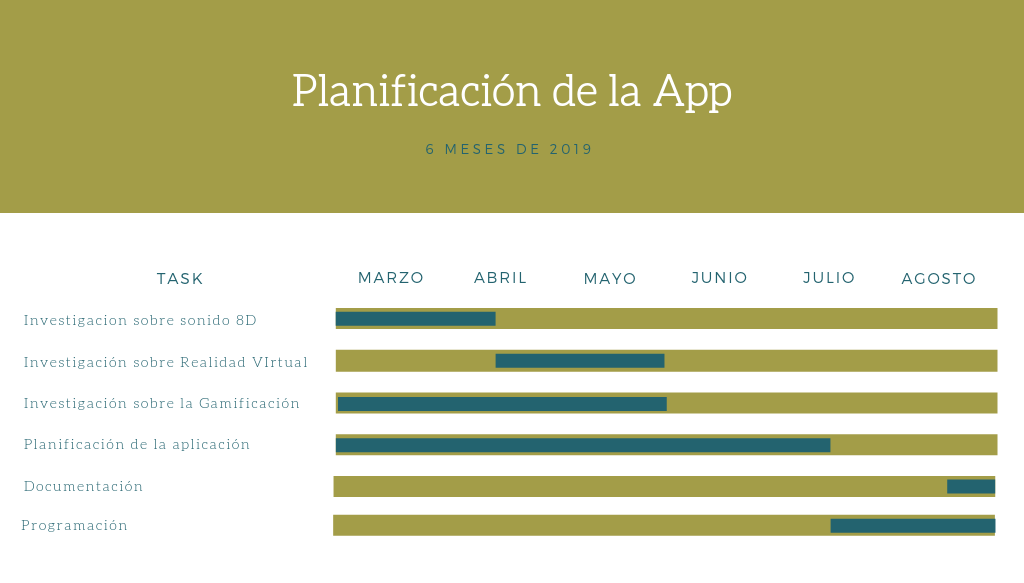
\includegraphics[width=1\textwidth]{./imagenes/diagramaGantt}
	\caption{Distribución del tiempo de desarrollo de la aplicación}
\end{figure}

\subsection{Costes e ingresos}

\quad Al no tener que pagar licencias de ningun programa utilizado, así como no necesitar comprar ningún aparato extra, la inversión monetaria en este proyecto ha sido cero.\\

\quad Por otro lado, la aplicación solo varía un poco un algoritmo ya existente, de forma que no se espera ningún tipo de beneficio por parte de esta aplicación, que solo es un campo de testeo para el algoritmo. \\

\quad Debido a que los algoritmos no se pueden patentar (al menos en España), tampoco se esperan beneficios de ningún tipo debidos a este factor.\\

\quad La intención de este proyecto era sin ánimo de lucro, por lo que al no haber tenido que invertir nada económicamente hablando ya hace que sea un balance positivo desde la perspectiva del desarrollador, quien solo ha invertido su tiempo y esfuerzo.\\ 

\newpage





	\thispagestyle{empty} 
	\textcolor[rgb]{1.00,1.00,1.00}{.} 
	\newpage %inserta un salto de página
	
	%--------------------------------------
	% ANALISIS
	%--------------------------------------
	
	\section{Análisis}

\subsection{Introducción}

\quad Aqui se analizarán las diferentes partes del proyecto agenas a la programación, como la investigación asociada al proyecto, o las herrramientas que se va a utilizar en el proyecto.\\ 

\subsection{Estado del arte}

\quad Aqui se van a analizar varios aspectos sobre el proyecto.\\

	\subsubsection{Sonido 8D}
\quad El audio 8D es la sensación de escuchar los sonidos a través de unos cascos en ángulos de trescientos sesenta grados, parecido a la realidad virtual.\\ 

\quad Este término que a resugido gracias a las redes sociales, dista de ser nuevo, ya que antiguamente era conocido como ambisonic, binaural o simplemente sonido 3D.\\

\quad Como estrategia de márketing, algunos músicos sugieren que la música danza alrededor de quien la escucha, provocando que muchos de los temas actuales, y no tan actuales, adquieran este sistema.\\

\quad A pesar de los avances, la sensación real y envolvente esta muy lejos de la realidad, ya que muchos elementos no se tiene en cuenta a la hora de determinar el posicionamiento del objeto. Por ejemplo, la transición entre delante y detrás del usuario pueden por momentos ser indistinguibles, ya que no se tienen de forma alguna en cuenta la orientación de las orejas, o el hecho de que si el usuario no se mueve, el cerebro humano no es capáz de distinguir entre una posición detante o detrás,asignando por defecto una posición delantera hasta que la fuente del sonido o el receptor se muevan, permitiendose entonces que el cerebro si situe en el espacio virtual.\\

\quad Ante este problema un desarrollador puede verse abrumado al principio, pero la solución a ambos problemas es más simple de lo que podría parecer, ya que en el caso de la orientación de las orejas es aplicar un coeficiente de division en los sonidos situados detrás del usuario, que se basa en el índice de ambsorción de sonido de la piel humana. En este caso se ha utilizado el de la goma para simular la piel. El según do problema no tiene una solución software a simple vista, pero teniendo en cuenta que el usuario interaccionará con el entorno moviendo la cabeza y avanzando por la escena, de forma que cambia su posición y horientación con respecto al foco, este problema se maquillara por la ppropia inmersión de la aplicación.\\ 

	\subsubsection{Realidad Virtual}
\quad Cuando hablamos de realidad virtual, hablamos de un entorno de apariencia real generado mediante tecnología informática que da la sensación de inmersión al usuario.\\ 

\quad Algunos centros educativos lo están usando para comprobar su viabilidad, sobre todo en casos de personas con dificultades en el aprendizaje, aunque presenta una serie de inconvenientes, como el coste o el espacio físico necesario para el usuario. A pesar de ello, se tienen grandes expectativas sobre su utilidad.\\

\quad Es importante añadir que en los últimos años hemos sufrido un boom con la aparición de la VR en el mundo del videojuego de una forma serie, sin embargo el precio de los equipos para los usuarios hace que los desarrolladores no inoven en este campo, por lo que si no se vuelven más económicos, algunos "expertos" afirman que podría desaparecer. \\

\quad Esta afirmación parece muy alarmista, ya que la VR no se utiliza solo en el hámbito del videojuego y se han hecho grandes avances para otros campos.\\

	\subsubsection{Gamificación}
\quad Se como el uso de diseños, elementos y características de juegos en contextos totalmente ajenos a estos. Socialmente hablando, especialmente a aquellos asiduos a las redes sociales, con los que comparten elementos como la lealtad del usuario, los logros o el reclutamiento a eventos con métodos atractivos y divertidos, dándoles una sensación de control y motivando su uso.\\

\quad Respecto a la educación, muchos han adoptado este estilo de enseñanza aunque no todos están de acuerdo. Su uso sigue expandiéndose cada vez más.\\

\quad En 2017, el Gobierno chino puso en marcha un enorme proyecto piloto en el ámbito social, basado en una especie de gamificación. Con ello, se cambió la magnitud y escala de lo que entendíamos por ‘gamificación’ , de tal manera que conectó la actividad online de sus ciudadanos con su estrategia social a gran escala, incorporándolos a un sistema de medición de conducta individual con ‘premios’ y ‘castigos’, a partir de un sistema de puntación llamada originalmente ‘crédito social’ que en origen, tenía propósitos comerciales relacionados con recompensas o incentivos.\\

\quad Esto no sería posible sin dos factores, la colaboración de grandes empresas chinas basadas en internet (como Alibaba, Baidu o Tencent) y las nuevas leyes de ciberseguridad chinas, que dan cobertura legal al acceso completo a casi todos los datos personales.\\

\subsection{Tecnologías y herramientas}

	\subsubsection{Lenguaje de programación C\#}

\quad Es un lenguaje de programación orientado a objetos desarrollado y estandarizado por Microsoft como parte de su plataforma .NET.\\

\quad Al ser un lenguaje orientado a objetos, admite los conceptos de encapsulación, herencia y polimorfismo. Todas las variables y métodos, incluido el método Main, el punto de entrada de la aplicación, se encapsulan dentro de las definiciones de clase. Una clase puede heredar directamente de una clase primaria, pero puede implementar cualquier número de interfaces. Los métodos que invalidan los métodos virtuales en una clase primaria requieren la palabra clave override como una manera de evitar redefiniciones accidentales. En C\#, un struct es como una clase sencilla; es un tipo asignado en la pila que puede implementar interfaces pero que no admite herencia.\\

\quad Escoger este lenguaje facilita el trabajo con unity, motivo por el cuál es el seleccionado.\\
	
	\subsubsection{GitKraken y GitHub}
	
\quad El uso de un repositorio y control de versiones es algo fundamental para llevar un control del trabajo en la aplicación, asi como poder volver a versiones anteriores del desarrollo en caso de ser necesario.\\

\quad GitKraken es una herramienta que tiene absolutamente todas las funcionalidades que se pueden llegar a querer en una herramienta para control de versiones con un rendimiento que deja en muy mal lugar al resto de herramientas (como SourceTree o Tortoise Git).\\

\quad Es la única herramienta que tiene versión de pago con su licencia PRO (49\$/año), sólo necesitarás esta licencia para un uso profesional o no comercial, pudiendo realizar tus proyectos personales con la versión gratuita sin ningún tipo de problemas, ya que las funcionalidades son las mismas.\\

\quad En cualquier caso, con la licencia de estudiante gratuita de GitHub se puede tener acceso a todas las funcionalidades, tanto de GitHub como de GitKraken.\\


	\subsubsection{Unity}

\quad Ha sido la opción para el desarrollo de la app. Ya hablamos de él en el apartado \textit{2.1.3. Comparativa de motores gráficos}.
	
	\subsubsection{Cardboard}

\quad Son un visor donde se coloca un teléfono móvil para experimentar una experiencia en realidad virtual.\\

\quad Actualmente google lo vende como experias en VR a bajo costo.\\

\newpage




	\thispagestyle{empty} 
	\textcolor[rgb]{1.00,1.00,1.00}{.} 
	\newpage %inserta un salto de página
	
	%--------------------------------------
	% DISENIO
	%--------------------------------------
	
	\section{Diseño}

\subsection{Visión global de la aplicación}

\quad La aplicación consta de tres escenas:\\

\begin{itemize}
	\item Init: donde la aplicación empieza.
	\item EchoChamber: donde se testeó el efecto del eco.
	\item Forest: donde se prueba el efecto del 8D con varios focos de sonido.
\end{itemize}

\quad Antes de empezar a hablar de cada uno de los elementos particulares de cada escena, es imperativo hablar de los elementos que son comunes en todas ellas. De este modo, en toda escena vamos a encontrar una serie de elementos que son imprescindibles: 
\begin{itemize}
	\item Foco de luz: configurado como luz direccional
	\item RealPlayer: contiene la cámara y la retícula y hace la función de representarnos en el mundo virtual
	\item GvrEditorEmulator: encargado de simular con el ratón el movimiento en modo VR
	\item GvrEventSystem: que se encarga de activar el input de colisión entre el rayo de detección que se emite desde la cámara por la retícula y los objetos con los que podemos interaccionar 
	\item SceneManager: se encarga de gestionar los eventos de salir de la aplicación y cambiar de escena
	item GvrControllerMain: se utiliza para determinar controles más allá del giro de cámara y el click, pero al final este elemento no se llegó a utilizar
\end{itemize}

\quad Ahora se pasa a hablar de las particularidades de cada escena.\\

\subsection{Escenas}
	\subsubsection{Init}
\quad Esta escena pretende poner en situación al usuario, indicando con un texto sobre una pared invisible como moverse y que es lo que tiene que hacer en ella.\\

\quad El objetivo será tan simple como encontrar el foco de sonido que lo está llamando. La voz para el foco ha sido aportada por Juan Hernández García, persona que menciono en los agradecimientos.\\

\begin{figure}[htb]
	\centering
	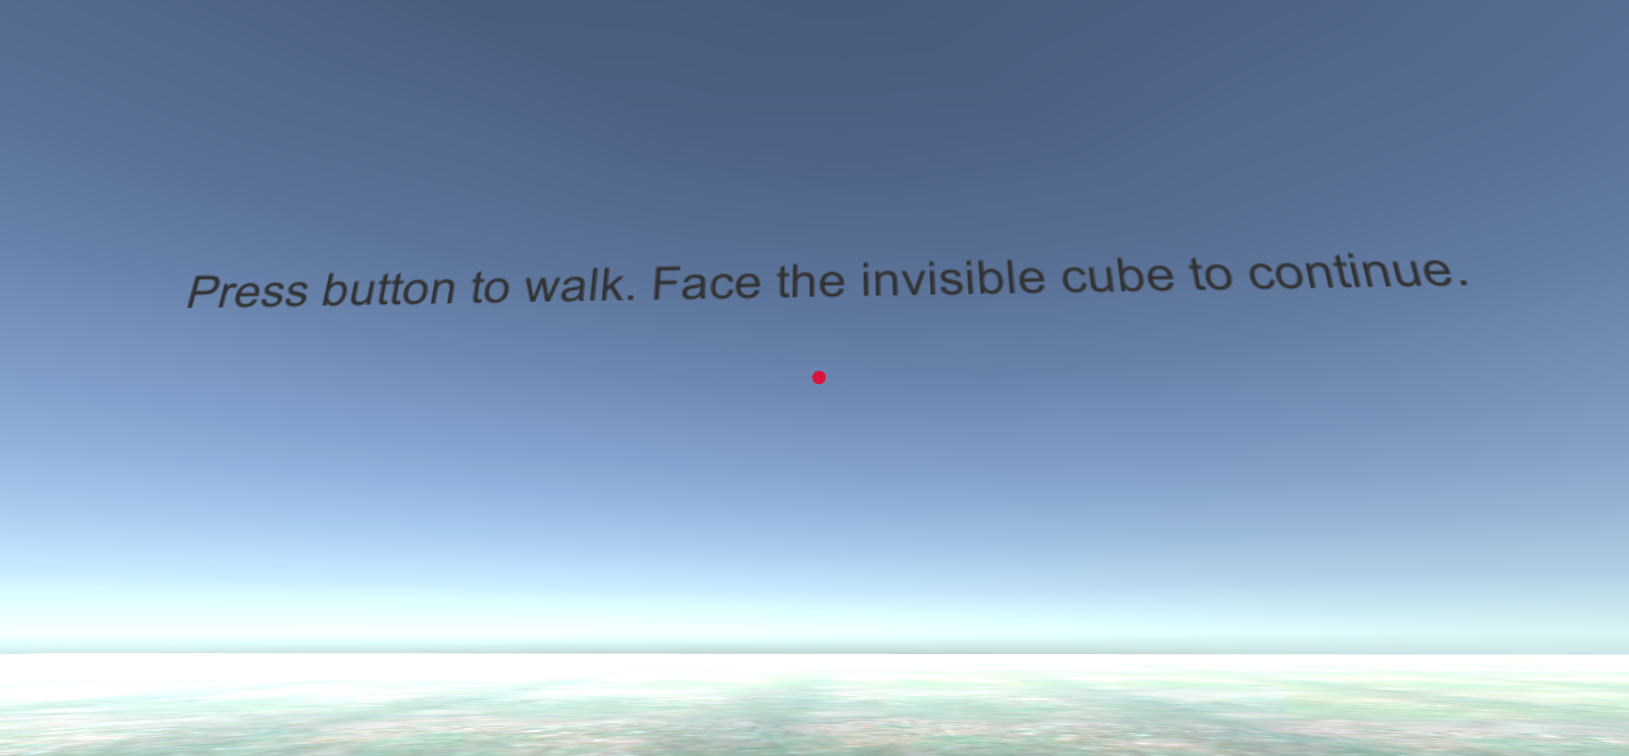
\includegraphics[width=0.6\textwidth]{./imagenes/initInstructions}
	\caption{Instrucciones de uso}
\end{figure}

\begin{figure}[htb]
	\centering
	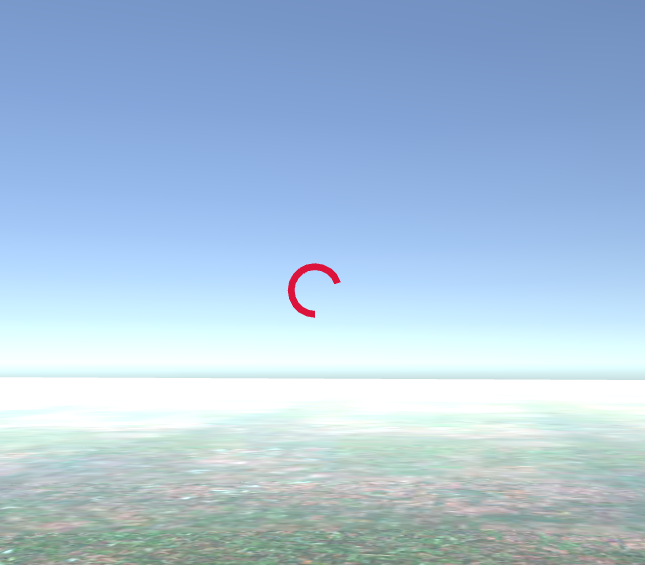
\includegraphics[width=0.248\textwidth]{./imagenes/inactiveCube}
	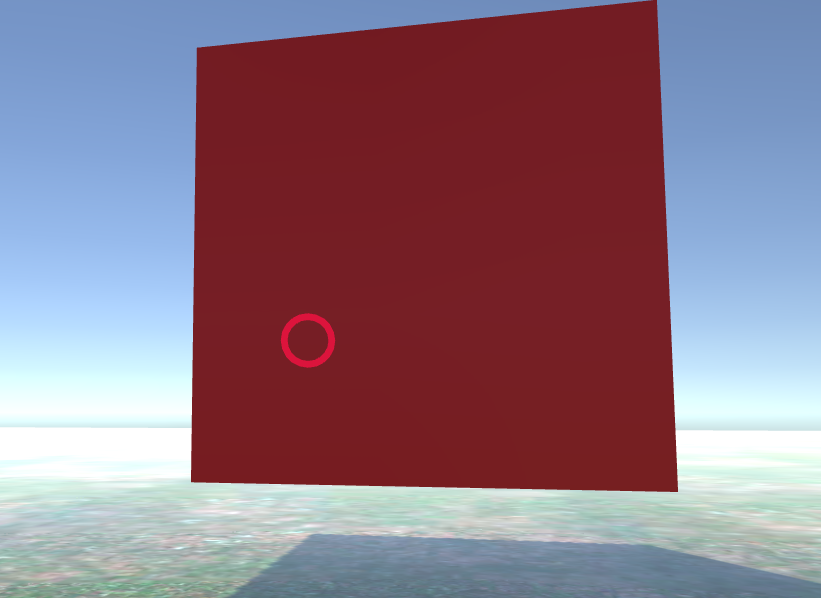
\includegraphics[width=0.3\textwidth]{./imagenes/activeCube}
	\caption{Cubo}
\end{figure}

\subsubsubsection{Componentes de Init}

\quad Dicho todo esto, toca hablar de cada uno de los elementos no comunes de la escena. De este modo, quedan por comentar los siguientes elementos:

\begin{itemize}
	\item Cube: sujeto que que se vuelve visible al encontrar su posición siguiendo el sonido de su llamada
	\item Plane: suelo de la escena
	\item Canvas: contiene un texto en que van unas pequeñas instrucciones
	\item Walls: Se forma con cuatro prismas invisibles que actuarán como muros invisibles para delimitar la zona de movimiento
\end{itemize}

	\subsubsection{EchoChamber}
\quad Esta habitación tiene como objetivo mostrar el efecto del eco ante un foco de sonido, en este caso será un icosaedro que toca la tonadilla libre de derechos \textit{If i had a chicken}, típica canción de taberna del oeste. Este icosaedro se tele transportará a otro lugar de la habitación cuando interactuemos con él.\\

\begin{figure}[htb]
	\centering
	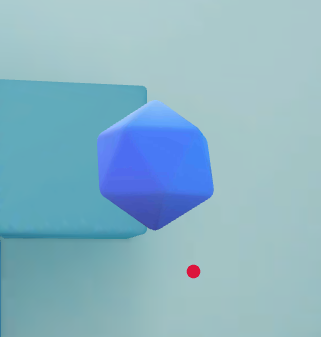
\includegraphics[width=0.4\textwidth]{./imagenes/icosaedroInactivo}
	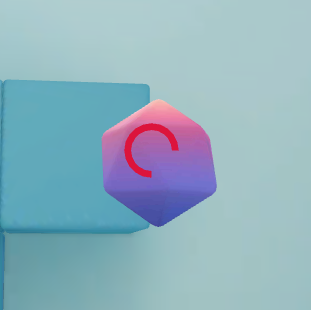
\includegraphics[width=0.4229\textwidth]{./imagenes/icosaedroActivo}
	\caption{Icosaedro sonoro}
\end{figure}

\quad Además, se encontrarán dos menús, unos con dos botones y otro con varios desplegables.\\

\quad Mediante el menú de dos botones se podrá salir de la aplicación o avanzar a la última escena. Además este menú contará con un texto que indique la utilidad de esta escena.\\

\begin{figure}[htb]
	\centering
	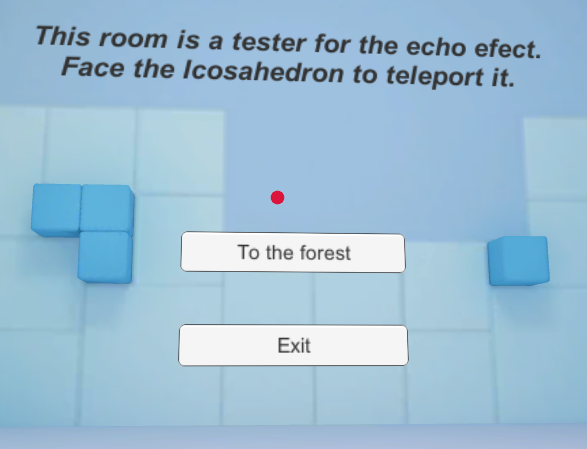
\includegraphics[width=0.5\textwidth]{./imagenes/echoMenu}
	\caption{Menú e instrucciones de la habitación}
\end{figure}

\quad El menú de desplegables se utiliza para para cambiar el tipo de material del que se componen las superficies de la habitación.\\

\begin{figure}[htb]
	\centering
	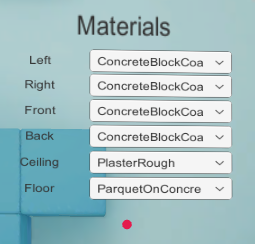
\includegraphics[width=0.3\textwidth]{./imagenes/materialMenu}
	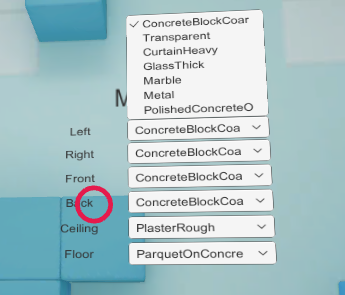
\includegraphics[width=0.3\textwidth]{./imagenes/materialMenuDeploy}
	\caption{Menú para cambio de materiales}
\end{figure}
\FloatBarrier

\subsubsubsection{Componentes de EchoChamber}
	
\quad Los elementos no comunes de la escena EchoChamber determinarán el comportamiento de la misma:
\begin{itemize}
	\item ResonanceAudioRoom: delimita la zona cúbica donde el eco puede trabajar. Si se sale de esta delimitación el eco desaparece
	\item CubeRoom: en esta escena se tiene una escena cúbica que delimita el espacio de interacción
	\item Menu: compuestos por dos botones (uno para avanzar de escena y otro para salir de la aplicación) y un texto que explica cómo funciona la escena.
\item Icosahedron: es el punto de sonido de la escena, y al interaccionar con él se teletransportará a un lugar aleatorio de la escena para poder observar cómo esto afecta al eco de la habitación
\item Canvas: este canvas tiene dentro una serie de dropdown que interaccionan directamente con ResonanceAudioRoom para modificar los diferentes materiales que que componen sus caras.
\end{itemize}

\quad En particular ResonanceAudioRoom, Icosahedron y Canvasson especialmente importantes, pues son los que permiten trabajar con el eco en esta habitación, pero no adelantemos acontecimientos.\\

	\subsubsection{Forest}

\quad Esta escena pretende representar un pequeño bosque lleno de pájaros que van cantando, volando por las cercanías.\\

\quad Dispone de un menú para volver a la escena EchoChamber o salir de la aplicación.\\

\begin{figure}[htb]
	\centering
	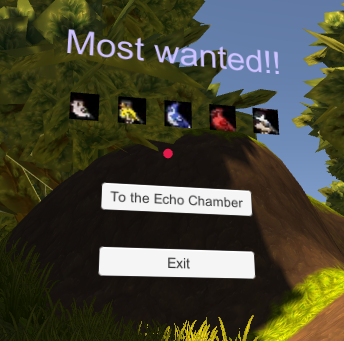
\includegraphics[width=0.36\textwidth]{./imagenes/forestMenu}
	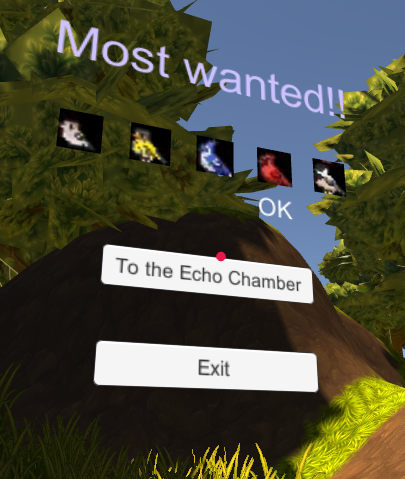
\includegraphics[width=0.38\textwidth]{./imagenes/forestMenuActive}
	\caption{Menú en el bosque}
\end{figure}

\quad En la parte superior del menú se encuentra un banner con los cinco pájaros dentro de la selección que se introduzcan en la aplicación. Cuando se visualice al tipo de pájaro objetivo, se marcará en ese banner.\\

\begin{figure}[htb]
	\centering
	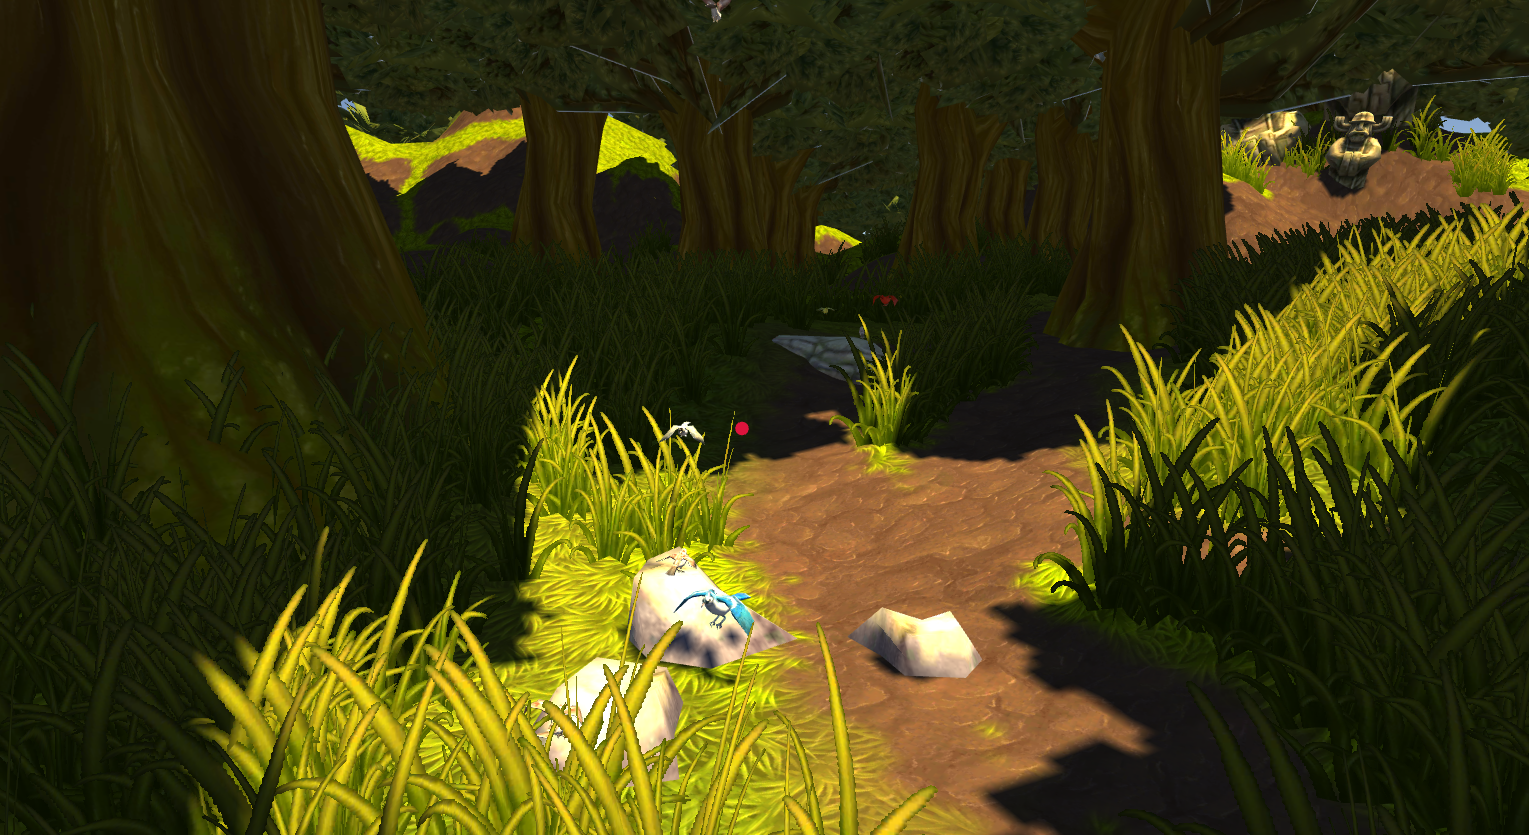
\includegraphics[width=0.7\textwidth]{./imagenes/forestBirds}
	\caption{Pajaros en el bosque}
\end{figure}

\quad Debido a la carga que tendrá esta escena, es importante cambiar shaders y aplicar técnicas de optimización para evitar que la tasa de frames caiga demasiado.

\begin{figure}[htb]
	\centering
	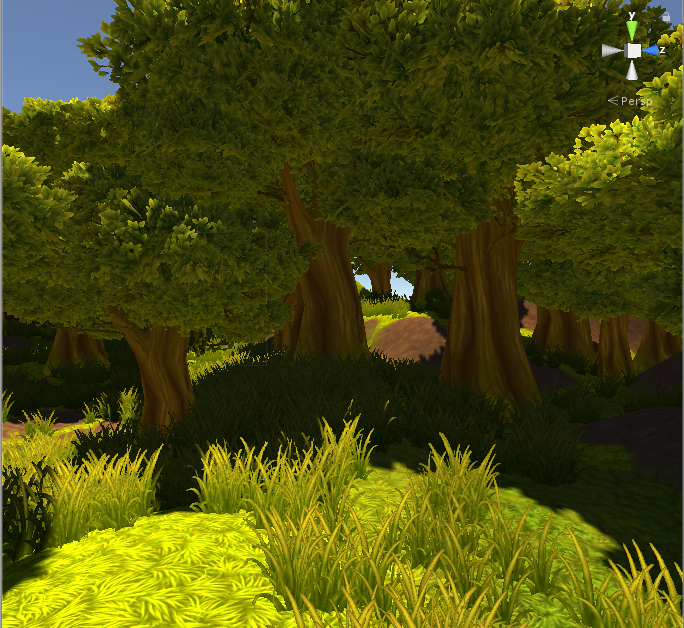
\includegraphics[width=0.45\textwidth]{./imagenes/highShadders}
	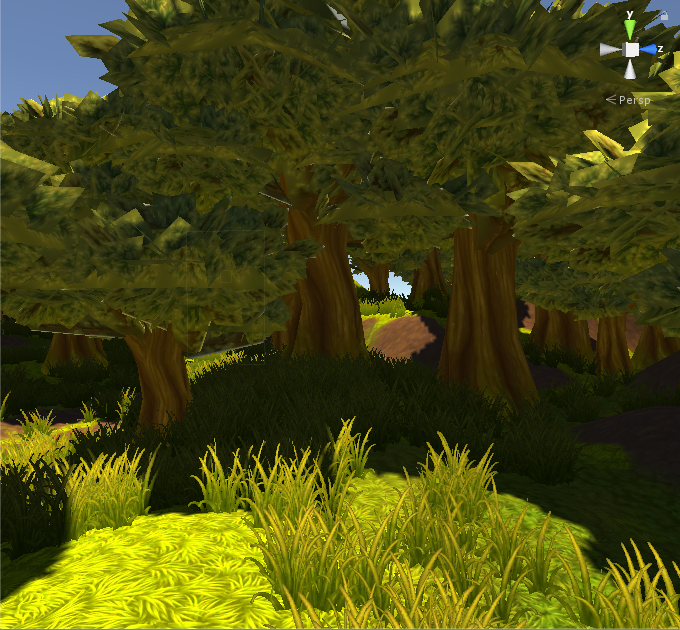
\includegraphics[width=0.45\textwidth]{./imagenes/lowShadders}
	\caption{Comparativa entre shader de alta calidad y baja calidad}
\end{figure}
\FloatBarrier

\subsubsubsection{Componentes de Forest}

\quad Forest es con diferencia la escena con más carga de elementos de todo el proyecto, por lo que voy a diferenciar entre tipos de elementos.\\

\quad Primero debemos se va a hablar de los elementos que tiene que ver con la topografía de las escena:

\begin{itemize}
	\item Terrain: terreno irregular que crearemos utilizando las herramientas de Unity. Aprovechando el asset Fantasy Forest, le agregaremos proceduralmente hierba y árboles
	\item Rock: Utilizaremos los dos tipos de rocas del asset Hand Painted Forest para dar algo de personalidad a nuestro bosque
	\item Statue: utilizaremos los modelados de estatuas del asset anteriormente nombrado para darle más personalidad al bosque
\end{itemize}

\quad Ahora pasamos a ver los elementos asociados al comportamiento de los pájaros:

\begin{itemize}
	\item \_livingBirdsController: se encarga de lanzar los distintos tipos de pájaros para que interaccionen por el bosque
	\item lc\_perchTarget: hace de objetivo donde los pájaros aterrizan, siempre que este no esté en el suelo
	\item lb\_GroundTarget: determina un lugar de aterrizaje para los pájaros en el suelo
\end{itemize}

\quad Una aclaración importante es que lc\_perchTarget y lb\_GroundTarget afectan de manera distinta al árbol de animaciones de los pájaros.\\

\quad Forest posee, al igual que Init, un conjunto de muros invisibles llamado Wall que determina la zona por la que el jugador puede moverse.\\ 

\quad El último tipo de elemento que queda por remarcar es un menú con con las mismas interacciones que tenía el de EchoChamber, pero con una particularidad, posee un banner encima suyo que determina si hemos visto o no los pájaros en el postrado.\\


\subsection{Modificaciones del algoritmo 8D}

\quad El algoritmo 8D clásico, a día del inicio de la parte práctica de este proyecto, presenta un problema fundamental a la hora de trabajar con un sonido al que se puede determinar la posición de su foco, y es que si el foco se mueve, la transición entre estar delante o detrás del usuario no se realiza de una forma correcta, dando la impresión de que el foco solo se está moviendo delante del usuario.\\

\begin{figure}[htb]
	\centering
	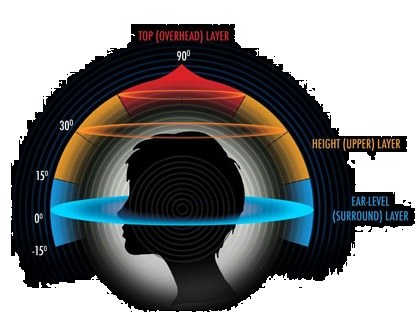
\includegraphics[width=0.7\textwidth]{./imagenes/8D}
	\caption{Percepción del algoritmo}
\end{figure}
\FloatBarrier

\quad Este problema se presenta, pues no se aplica un factor de reducción del sonido que tenga en cuentas dos factores determinantes a la hora del cálculo, que el ser humano tiene orejas que están orientadas, y que además estas poseen un factor de absorción del sonido, de forma que no deben bloquearlo totalmente, si no reducirlo en función de este factor.\\

\quad Para determinar esto y aplicarlo al algoritmo con el que nos encontramos, solo deberemos tener en cuenta que ahora no tenemos un solo vector de orientación para la cámara a la hora determinar la posición de los sonidos en la parte trasera de la cabeza del usuario, si no que debemos hacer una discriminación  los cálculos, sabiendo que la orientación de la oreja afecta a la percepción del sonido, de forma que el cálculos de los vectores que determinan la llegada debe variar aplicando así una reducción extra en la intensidad con la que se percibe.\\

\quad Ahora toca hablar sobre la reducción de sonido que plantea la oreja no por su orientación, si no por su materia.\\

\quad Los cambios efectuados por esto se aplican los últimos, ya que solo afecta a la zona trasera de la cabeza. Teniendo en cuenta el factor de absorción de sonido de la piel humana, que en este caso se ha equiparado al de la goma, se divide el resultado si se encuentra el foco en la zona designada.\\


\begin{figure}[htb]
	\centering
	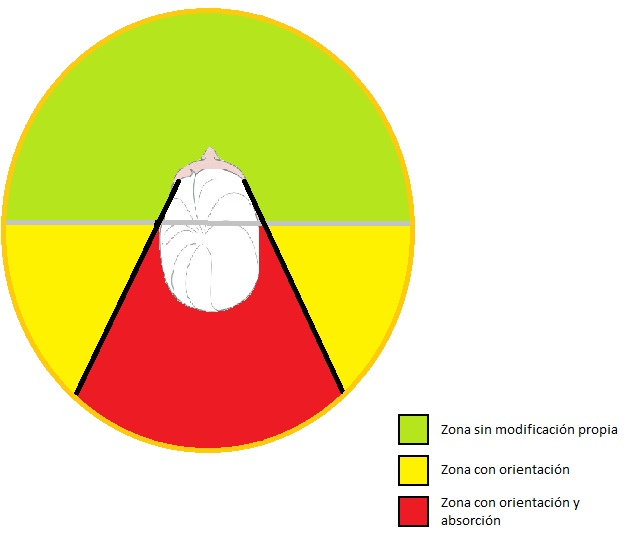
\includegraphics[width=0.7\textwidth]{./imagenes/zonasAlgoritmo}
	\caption{Zonas del algoritmo}
\end{figure}
\FloatBarrier

\newpage






	\thispagestyle{empty} 
	\textcolor[rgb]{1.00,1.00,1.00}{.} 
	\newpage %inserta un salto de página
	
	%--------------------------------------
	% IMPLEMENTACION
	%--------------------------------------
	
	\section{Implementación y control de versiones}

\subsection{Introducción}

\quad En esta parte se presentan las diferentes implementaciones necesarias, así como un control de versiones de la aplicación en la que desmenuzaremos las diferentes versiones. \\

\quad Llevar un control de versiones es esencial como desarrollador, por lo que para este fin utilizo la página \textit{github}, y como herramienta secundaria para la gestión del repositorio, utilizo \textit{GitKraken}. Para el desarrollo de esta aplicación se ha seguido el paradigma de \textit{GitFlow} a la hora del control de versiones con el repositorio.\\
 
\subsection{GitFlow}
\subsubsection{¿Qué es GitFlow?}

\quad Gitflow es un diseño de flujo de trabajo Git que se publicó por primera vez y se hizo popular por \textit{Vincent Driessen} en \textit{nvie}. El flujo de trabajo de Gitflow define un modelo de ramificación estricto diseñado en torno al lanzamiento del proyecto. Esto proporciona un marco robusto para gestionar proyectos más grandes.\\

\quad Gitflow es ideal para proyectos que tienen un ciclo de lanzamiento programado, pues este flujo de trabajo no agrega nuevos conceptos o comandos más allá de lo que se requiere para el Flujo de trabajo de la rama de funciones, si no que asigna roles muy específicos a diferentes ramas y define cómo y cuándo deben interactuar. Además de las ramas de características, utiliza ramas individuales para preparar, mantener y grabar lanzamientos. Por supuesto, también puede aprovechar todos los beneficios del flujo de trabajo de Branch Branch: solicitudes de extracción, experimentos aislados y una colaboración más eficiente.\\ 

\subsubsection{¿Cómo funciona?}

\subsubsubsection{Ramas Develop \& Master}

\quad En lugar de una sola rama, este flujo de trabajo usa dos ramas para registrar el historial del proyecto.\\ 

\quad La rama \textit{master} almacena el historial de lanzamiento oficial, y la rama \textit{develop} sirve como una rama de integración de características. También es conveniente etiquetar todos los commits en master con un número de versión.\\

\begin{figure}[htb]
	\centering
	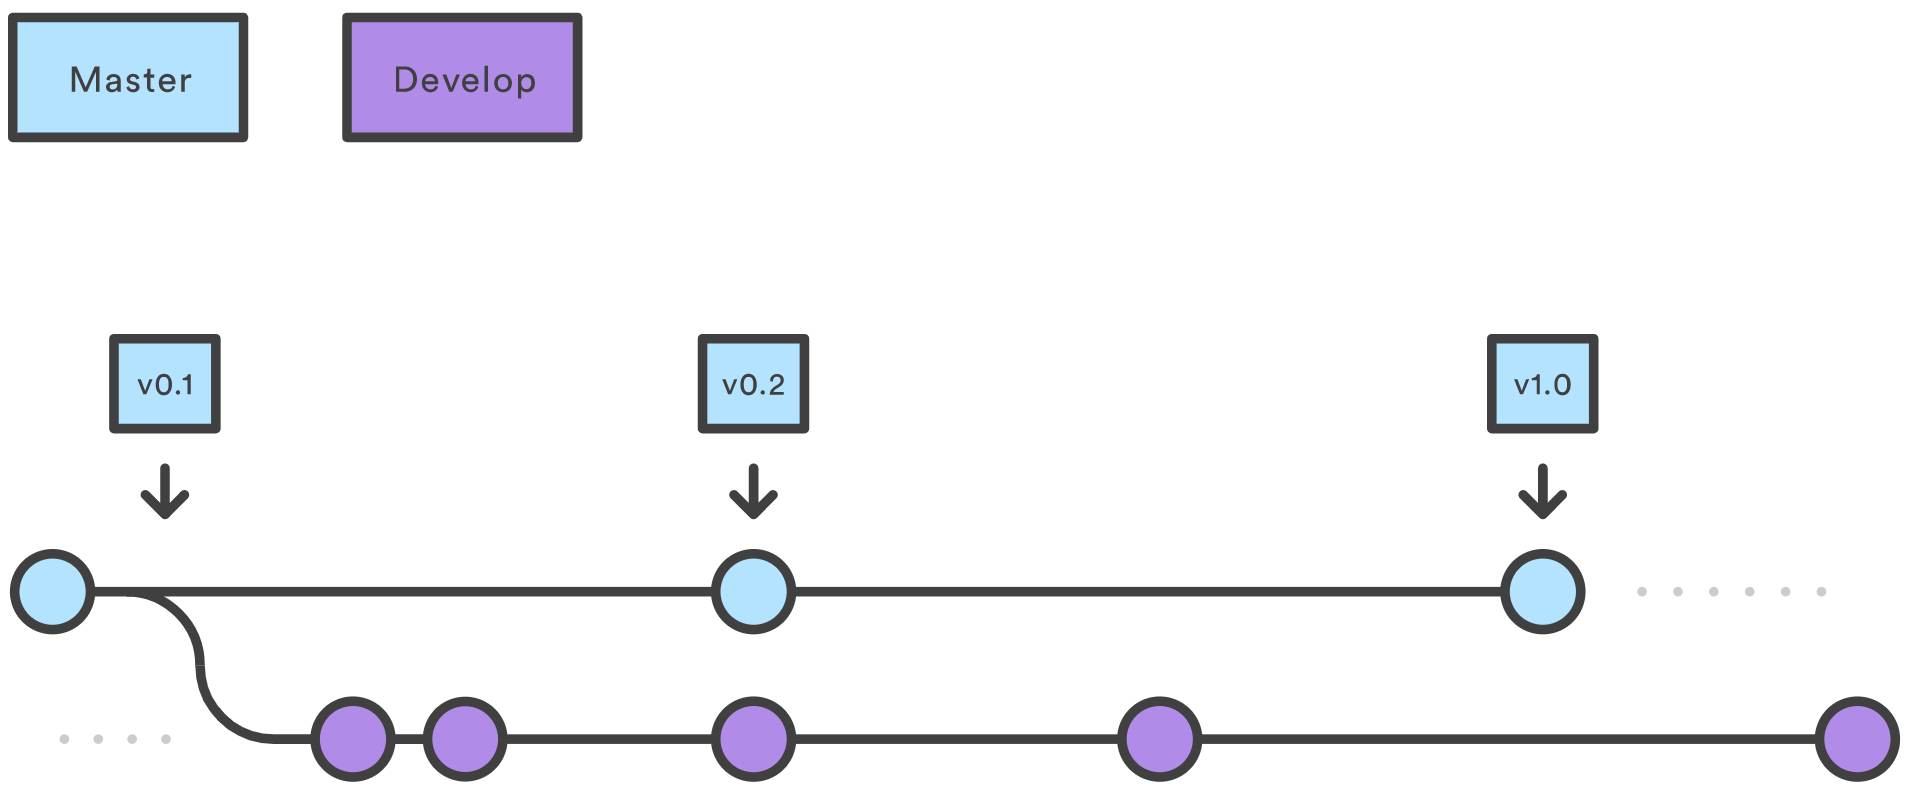
\includegraphics[width=0.75\textwidth]{./imagenes/master-dev}
	\caption{Ramas Develop y Master}
\end{figure}

\subsubsubsection{Ramas Feature}

\quad Cada nueva feature debe residir en su propia rama, que se puede enviar al repositorio central como respaldo/colaboración.\\

\quad En lugar de bifurcarse de master, las features usan el desarrollo como su rama principal, de forma que cuando se completa una característica, se fusiona nuevamente en develop. Las características nunca deberían interactuar directamente con el maestro.\\

\begin{figure}[htb]
	\centering
	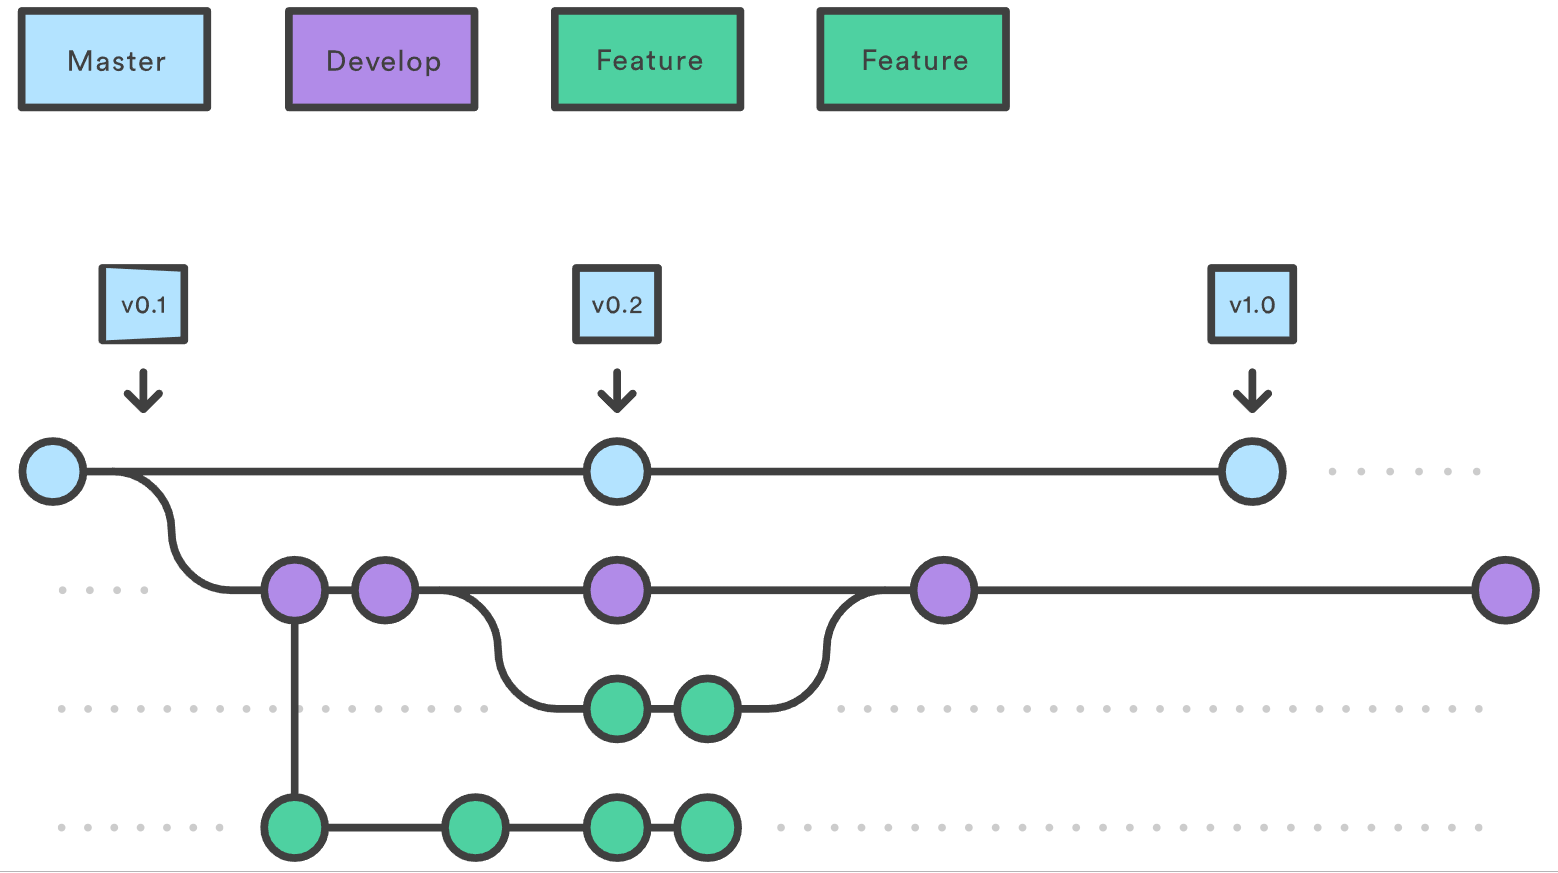
\includegraphics[width=1\textwidth]{./imagenes/feature}
	\caption{Rama feature}
\end{figure}

\subsubsubsection{Ramas Release}

\quad Una vez que el desarrollo ha adquirido suficientes características para un lanzamiento,  bifurca una rama de release fuera del desarrollo. La creación de esta rama inicia el siguiente ciclo de lanzamiento, por lo que no se pueden agregar nuevas características después de este punto. Solo las correcciones de errores, la generación de documentación y otras tareas orientadas a la versión deben ir en esta rama.\\ 

\quad Una vez que está listo para enviar, la release se fusiona en master y se etiqueta con un número de versión. Además, debe fusionarse nuevamente en el desarrollo, que puede haber progresado desde que se inició el lanzamiento.\\

\begin{figure}[htb]
	\centering
	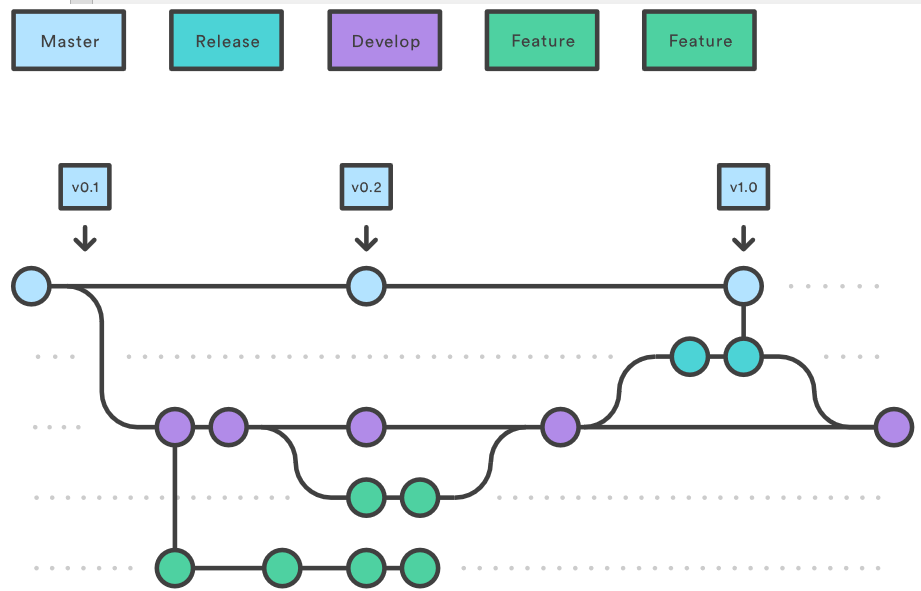
\includegraphics[width=1\textwidth]{./imagenes/release}
	\caption{Rama release}
\end{figure}

\subsubsubsection{Ramas Hotfix}

\quad Las ramas de mantenimiento o "hotfix" se utilizan para parchear rápidamente las versiones de producción.\\

\quad Las ramificaciones de revisión son muy parecidas a las ramificaciones de lanzamiento y ramificaciones de características, excepto que se basan en master en lugar de develop.\\

\quad Esta es la única rama que debe bifurcarse directamente de master, y tan pronto como se complete la corrección, debe fusionarse tanto en master como en develop (o en la rama de la versión actual), y master debe etiquetarse con un número de versión actualizado.\\

\begin{figure}[htb]
	\centering
	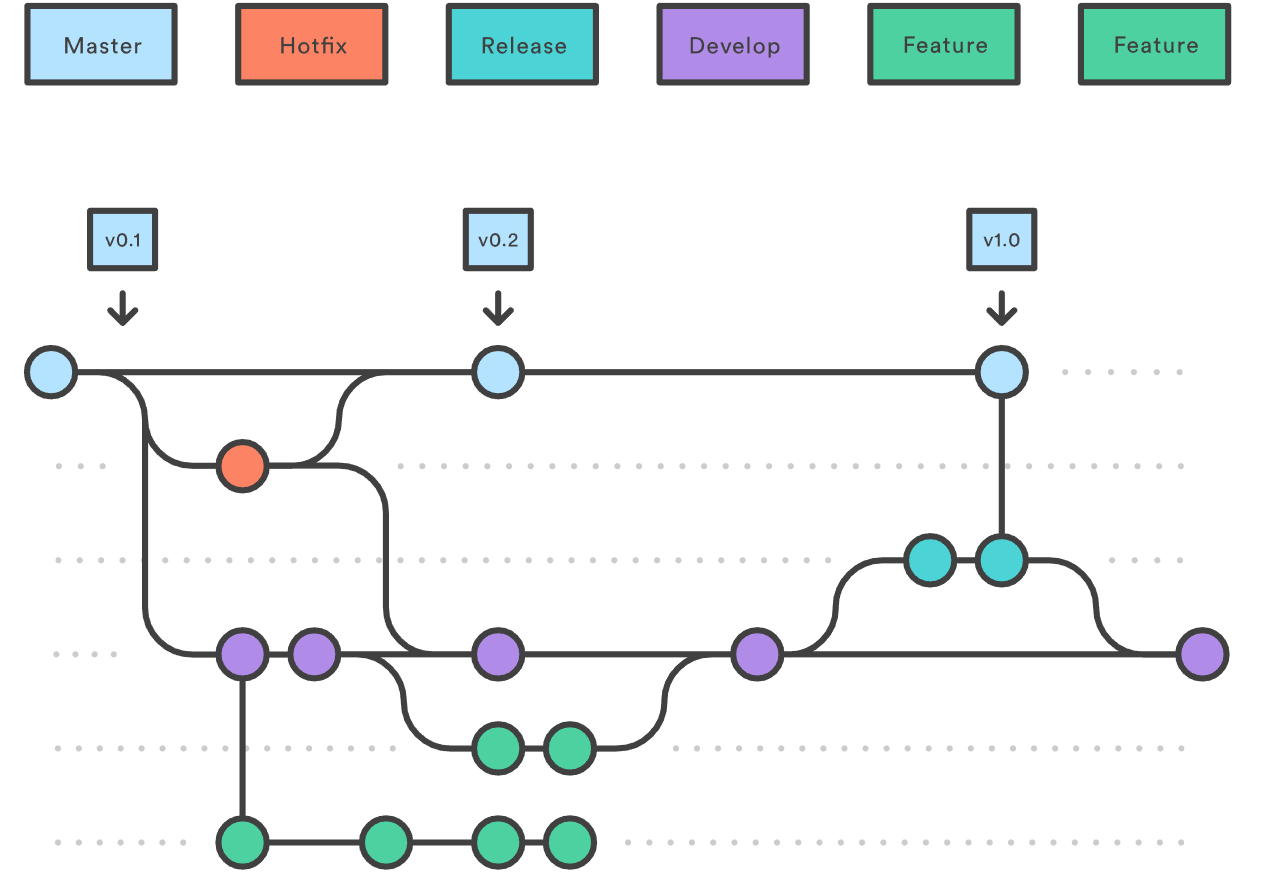
\includegraphics[width=0.6\textwidth]{./imagenes/hotfix}
	\caption{Rama hotfix}
\end{figure}

\subsection{Control de versiones}

\quad A continuación, se presenta el árbol de desarrollo de la aplicación en las que se ve un resumen de las modificaciones:\\

\begin{figure}[htb]
	\centering
	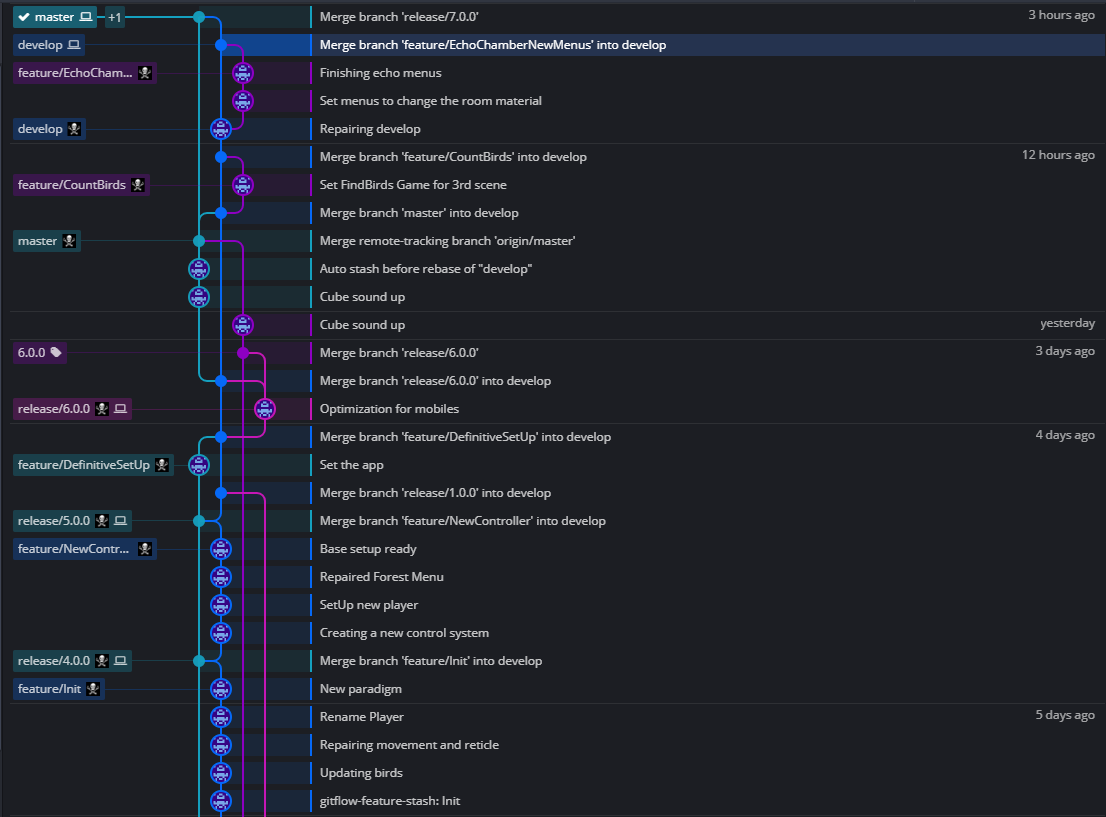
\includegraphics[width=0.7\textwidth]{./imagenes/git-tree1}
	\caption{Primera mitad del árbol de flujo del repositorio}
\end{figure}

\begin{figure}[htb]
	\centering
	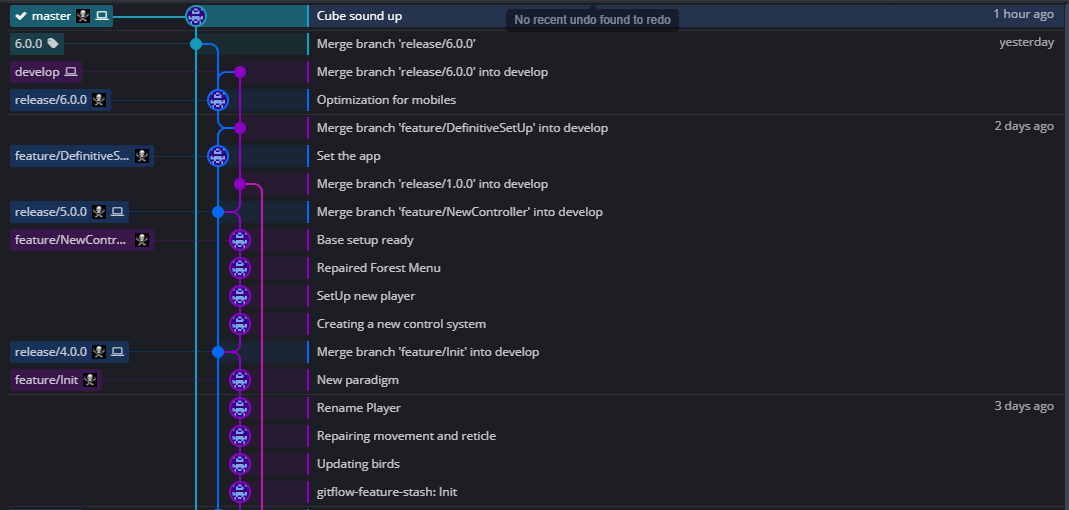
\includegraphics[width=0.7\textwidth]{./imagenes/git-tree2}
	\caption{Segunda mitad del árbol de flujo del repositorio}
\end{figure}

\subsubsection{Cambios en el paradigma de interacción del usuario}

\quad El desarrollo de una aplicación no es ni mucho menos algo estático que sigue estrictamente los pasos definidos al inicio de éste durante la planificación. Un buen desarrollo debe saber adaptarse a requisitos que pudieron no tenerse en un principio.\\

\quad Este es el caso de la aplicación aqui presentada, de forma que me dispongo a enumerar unos cuantos cambios que surgieron a lo largo del desarrollo y que merecente ser resaltados por encima de los demás:\\

\begin{itemize}
	\item En la versión 5.0.0, desecho un control del movimiento del personaje basado en mando por un control basado únicamente en los que el cardboard nos presenta, pasando el botón de pantalla a a haber que el personaje se mueva hacia adelante, y las interacciones con elementos de las escenas presentadas con un cargador de tiempo. Este cambio surge al plantearme facilitar el uso para el usuario, al no depender de otro dispositivo externo, en este caso un mando.
	\item En la versión 6.0.0 la reticula de carga pasa a ser la propia reticula puntero que utiliza. Esto se realiza con la idea de evitar que la superposición de ambas retículas pueda marear al usuarion cuando la de carga entra en escena.
	\item  En la versión 6.0.0 se aplica oclussion culling en la escena del bosque. Esto se hace para reducir su carga y así maximizar los frames de la escena.
\end{itemize}

\subsection{Implementación general: setUp de la aplicación}

\quad El trabajo de esta aplicación se ha desarrollado con Unity 2018.4.6f1. Esto se ha hecho así debido a que el hub de Unity determinaba que esta era la última versión estable de la aplicación en el momento del inicio de la programación de este proyecto.\\

\quad Deberemos configurar también la sdk para que Unity pueda trabajar. Normalmente si ya se tiene la sdk de android instalada, Unity la reconocerá sin necesidad de añadirla manualmente.\\

\quad Debemos tener en cuenta que, en "Edit>Project Settings", debemos activar la casilla \textit{Virtual Reality Supported} de XR Settings para android en el "Player", y fijar en la pestaña "Other Settings" el \textit{Minimum API Leve} a nivel 19.\\

\subsubsection{Paquetes a descargar}

\quad Los paquetes que necesitaremos para poder utilizar la tecnología necesaria en Unity son:\\

\begin{itemize}
	\item ResonaceAudioForUnity\_<versión\_deseada>.unitypackage
	\item GoogleVRForUnity\_<versión\_deseada>.unitypackage
\end{itemize}

\quad Para instalar un paquete, introduciremos el paquete en cuestión desde la pestaña "Assets>Import Package>Custom Package".\\

\subsection{Jugador}

\quad El jugador estará formado por un GameObject llamado \textit{RealPlayer} que contendrá la "MainCamera". Se introducirá como hijo de ésta el prefab \textit{GvrReticlePointer} que pondrá en el jugador la reticula que utilizaremos para las iteracciones. Hay una serie de cambios en la retícula que se explican en el siguiente subapartado.\\

\begin{figure}[htb]
	\centering
	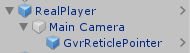
\includegraphics[width=1\textwidth]{./imagenes/player}
	\caption{Aspecto del Jugador en el árbol de escena}
\end{figure} 

\subsubsection{Controles de movimiento}

\quad Se ha implementado para el movimiento que cuando se hace click en la pantalla, el jugador se mueve. Esto se consigue añadiendo un script de C\# a \textit{RealPlayer} que contendra el siguiente código:

\lstset{language=[sharp]C, breaklines=true, basicstyle=\footnotesize}
\begin{lstlisting}[frame=single, caption={PlayerWalk.cs}]
using System.Collections;
using System.Collections.Generic;
using UnityEngine;

public class PlayerWalk : MonoBehaviour
{
    public int playerSpeed;

    // Update is called once per frame
    void Update()
    {
        if (Input.GetButton("Fire1")) {
            transform.position = transform.position + Camera.main.transform.forward * playerSpeed * Time.deltaTime;
        }
    }
}
\end{lstlisting}

\subsubsection{Control de cámara en VR}

\quad Simplemente se añadirá al árbol de escena el prefab de GoogleVR \textit{GvrEditorEmulator}.

\subsubsection{Retícula}

\quad La retícula que viene por defecto en unity no será necesaria en el caso presentado, pues es mejor y más eficiente utilizar el script \textit{GvrPointerPhysicsRaycaster.cs}, adjunto con el paquede de GoogleVR.\\

\quad La retícula es el medio para interactuar con el medio, pero no interesa que se active automáticamente, si no que será preciso que haya un tiempo de espera para que el usuario decida si se va a llevar a cavo esta interacción o si por el contrario desea canscelarla.\\

\quad Con motivo de ello, se aprobechará la capacidad de la retícula de google de ampliarse en una iteracción (efecto producido con el prefab \textit{GvrEventSystem}.) y se modificará el angulo mostrado en pantalla de ésta el cuál se irá modificando, convirtiendola así en una barra de carga circular. Para esto se requieren las siguientes modificaciones en el shader de Google:

\begin{itemize}
	\item Añadir la propiedad Angle
	\item Añadir el float que la representará
	\item Sustituir la función \textit{vert} para para que tenga en cuenta esta nueva propiedad en el shader 
\end{itemize}

\quad A continuación se adjunta el resultado final para ver como debe quedar el código:

\lstset{language=[sharp]C, breaklines=true, basicstyle=\footnotesize}
\begin{lstlisting}[frame=single, caption={GvrReticleShader.shader}]
// Copyright 2015 Google Inc. All rights reserved.
//
// Licensed under the Apache License, Version 2.0 (the "License");
// you may not use this file except in compliance with the License.
// You may obtain a copy of the License at
//
//     http://www.apache.org/licenses/LICENSE-2.0
//
// Unless required by applicable law or agreed to in writing, software
// distributed under the License is distributed on an "AS IS" BASIS,
// WITHOUT WARRANTIES OR CONDITIONS OF ANY KIND, either express or implied.
// See the License for the specific language governing permissions and
// limitations under the License.

Shader "GoogleVR/Reticle" {
  Properties {
    _Color  ("Color", Color) = ( 1, 1, 1, 1 )
    _InnerDiameter ("InnerDiameter", Range(0, 10.0)) = 1.5
    _Angle("Angle", Range(0, 360)) = 180
    _OuterDiameter ("OuterDiameter", Range(0.00872665, 10.0)) = 2.0
    _DistanceInMeters ("DistanceInMeters", Range(0.0, 100.0)) = 2.0
  }

  SubShader {
    Tags { "Queue"="Overlay" "IgnoreProjector"="True" "RenderType"="Transparent" }
    Pass {
      Blend SrcAlpha OneMinusSrcAlpha, OneMinusDstAlpha One
      AlphaTest Off
      Cull Back
      Lighting Off
      ZWrite Off
      ZTest Always

      Fog { Mode Off }
      CGPROGRAM

      #pragma vertex vert
      #pragma fragment frag

      #include "UnityCG.cginc"

      uniform float4 _Color;
      uniform float _InnerDiameter;
      uniform float _OuterDiameter;
      uniform float _DistanceInMeters;
      uniform float _Angle;

      struct vertexInput {
        float4 vertex : POSITION;
      };

      struct fragmentInput{
          float4 position : SV_POSITION;
      };

  /*    fragmentInput vert(vertexInput i) {
        float scale = lerp(_OuterDiameter, _InnerDiameter, i.vertex.z);

        float3 vert_out = float3(i.vertex.x * scale, i.vertex.y * scale, _DistanceInMeters);

        fragmentInput o;
        o.position = UnityObjectToClipPos (vert_out);
        return o;
      }
*/
      fragmentInput vert(vertexInput i) {
	  fragmentInput o;
	  if (_DistanceInMeters < 20) {
		  // 180* = 2.9
		  // limit = - (a - 180) * 2.9/180
		  float limit = -(_Angle - 180) * 0.0161111111;
		  float3 vert_out = float3(0, 0, _DistanceInMeters);
		  float a = -atan2(i.vertex.x, i.vertex.y);
		  if (a >= limit) {
			  float scale = lerp(_OuterDiameter, _InnerDiameter, i.vertex.z);
			  vert_out = float3(i.vertex.x * scale, i.vertex.y * scale, _DistanceInMeters);
		  }
		  o.position = UnityObjectToClipPos(vert_out);
	  }
	  return o;
}

      fixed4 frag(fragmentInput i) : SV_Target {
        fixed4 ret = _Color;
        return ret;
      }

      ENDCG
    }
  }
}

\end{lstlisting}

\subsubsubsection{Interacción de la retícula}

\quad Ahora entra en juego como conseguir la interacción con el objeto. Para ello se requieren dos pasos muy importantes: \\

\begin{itemize}
	\item Añadir al objeto un \textit{EventTrigger} que trabajará cuando el puntero entre dentro del area que ocupa el objeto y cuando salga.
	\item Añadir un script al objeto que en este caso se ha llamdo \textit{GVRButton.cs}.
\end{itemize}

\quad lo primero debe hacerle para determinar las fundiones GvrOn y GvrOff que determinarán el comportamiento ante la entrada y la salida del objeto. El segundo determina la acción que se llevará a cabo a partir de que termine el evento de entrada, que en este caso que la barra de carga termine de llenarse.\\

\quad Se adjuntan seguidamente es aspecto de un objeto que posee estas cualidades y el código asociado a \textit{GVRButton.cs}.\\

\begin{figure}[htb]
	\centering
	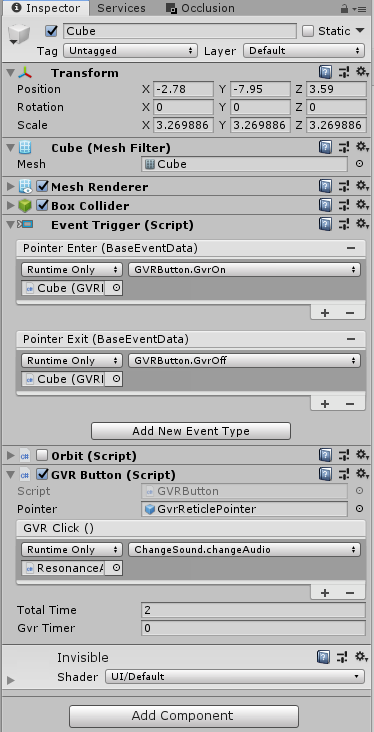
\includegraphics[width=0.35\textwidth]{./imagenes/cube}
	\caption{Cubo con interacciones}
\end{figure} 

\lstset{language=[sharp]C, breaklines=true, basicstyle=\footnotesize}
\begin{lstlisting}[frame=single, caption={GVRButton.cs}]
using System.Collections;
using System.Collections.Generic;
using UnityEngine;
using UnityEngine.UI;
using UnityEngine.Events;

public class GVRButton : MonoBehaviour
{
    public GameObject pointer;
    public UnityEvent GVRClick;
    public float totalTime = 2;
    bool gvrStatus;
    public float gvrTimer;
    Renderer rend;
    float angle;

    private void Start()
    {
        rend = pointer.GetComponent<Renderer>();
    }

    // Update is called once per frame
    void Update()
    {
        if (gvrStatus)
        {
            gvrTimer += Time.deltaTime;
            angle= gvrTimer / totalTime * 360;
            rend.material.SetFloat("_Angle", angle);
        }

        if (gvrTimer > totalTime)
        {
            GVRClick.Invoke();
        }
    }

    public void GvrOn()
    {
        gvrStatus = true;
    }

    public void GvrOff()
    {
        gvrStatus = false;
        gvrTimer = 0;
        rend.material.SetFloat("_Angle", 360f);
    }
}

\end{lstlisting}

\quad En el código se muestra como acceder al shader y modificar el ángulo que creamos en el apartado anterior dentro de la función update.\\

\subsubsection{Aplicar sonido 8D a un objeto}

\quad Esta parte se soluciona rápidamente añadiendo los dos siguientes elementos al objeto emisor de sonido y a la mainCamera:\\

\begin{itemize}
	\item El script \textit{ResonanceAudioListener.cs} a la main camera de la escena.
	\item El prefab\textit{ResonanceAudioSource} al objeto que hará de emisor.
\end{itemize}

\quad Es importante añadir el audio que queremos que se reproduzca en la propiedad \textit{Audio Source} para que los scripts puedan trabajar.\\

\begin{figure}[htb]
	\centering
	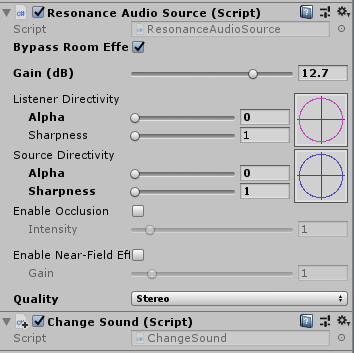
\includegraphics[width=0.5\textwidth]{./imagenes/audiosource}
	\caption{Script ResonaceAudioSource}
\end{figure} 

\begin{figure}[htb]
	\centering
	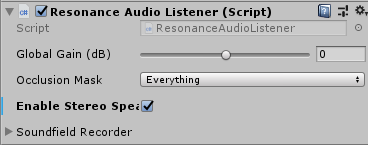
\includegraphics[width=0.5\textwidth]{./imagenes/audiolistener}
	\caption{Script ResonaceAudioListener}
\end{figure} 

\subsection{Implementación por escenas}

\quad Ahora analizaremos los detalles más importantes implementados por escena.\\
 
	\subsubsection{Escena Init}
		\subsubsubsection{Cubo para interactuar}

\quad Ya se ha hablado de el cubo de la pimera escena que interactua con el usuario cuando lo mira, pero tiene varias acciones que realizar en el momento de la iteracción:\\

\begin{itemize}
	\item Cambiar el audio que se esta reproduciendo durante la ejecución.
	\item Cambiar la escena en la que se encuentra el jugador.
	\item Cambiar el material del cubo para que se haga visible.
\end{itemize}

\quad La primera acción requiere que por nuestra parte creemos un script que active la subrutina que cambie en ejecución el audio reproducido. La segunda accíon requiere que cuando se termine de reproducir el nuevo audio se cargue la siguiente escena. El siguiente código muestra como hacer ambas cosas desde la subrutina WaitFinish:\\

\lstset{language=[sharp]C, breaklines=true, basicstyle=\footnotesize}
\begin{lstlisting}[frame=single, caption={ChangeSound.cs}]
using System.Collections;
using System.Collections.Generic;
using UnityEngine;
using UnityEngine.SceneManagement;
using UnityEngine.Timeline;

public class ChangeSound : MonoBehaviour
{
    AudioSource myaudio;
    Material mymaterial;
    Renderer rend;

    public void changeAudio()
    {
        mymaterial = Resources.Load<Material>("RedMat");
        rend = GetComponentInParent<Renderer>();
        rend.enabled = true;
        rend.sharedMaterial = mymaterial;
        StartCoroutine(WaitFinish());
    }

    IEnumerator WaitFinish()
    {
        myaudio = GetComponent<AudioSource>();
        //myaudio.Stop();
        myaudio.clip = Resources.Load<AudioClip>("porfinteveo3");
        myaudio.Play();
        yield return new WaitForSeconds(myaudio.clip.length);
        SceneManager.LoadScene("EcoChamber");
    }
}

\end{lstlisting}

\quad En el mismo código se incluye dentro de la función changeAudio el método para poder cambiar el material de un GameObject.\\

	\subsubsection{Escena Echo Chamber}
		\subsubsubsection{Aplicar eco}
\quad Dentro del GameObject que define la habitación se debe añadir el prefab ResonanceAudioRoom, modificando el tamaño de este para que se ajuste al tamaño de la habitación.

\begin{figure}[htb]
	\centering
	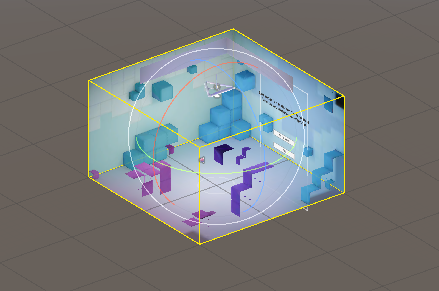
\includegraphics[width=1\textwidth]{./imagenes/echoroom}
	\caption{ResonanceAudioRoom ajustado a la habitación de la escena}
\end{figure} 

\quad Desde el script asociado al prefab, se pueden modificar los materiales que componen las dicerentes caras del cubo que delimita el espacio que dispondrá de eco, así como las características del eco en cuestión (reflectividad, tiempo, ganancia en DB, brillo).\\

\begin{figure}[htb]
	\centering
	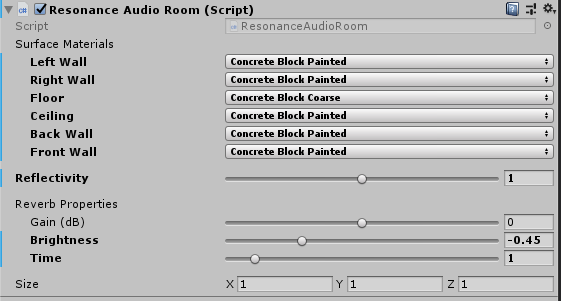
\includegraphics[width=1\textwidth]{./imagenes/audioroom}
	\caption{Script ResonaceAudioRoom}
\end{figure}

		\subsubsubsection{Icosaedro el sonido}

\quad Respecto al icosaedro solo queda añadir la función que lo hace teleportarse cuando el evento entra en acción. Esta función se recoge en el siguiente código:\\

\lstset{language=[sharp]C, breaklines=true, basicstyle=\footnotesize}
\begin{lstlisting}[frame=single, caption={Teleporter.cs}]
using System.Collections;
using System.Collections.Generic;
using UnityEngine;

public class Teleporter : MonoBehaviour
{

    Vector3 destination;
    RectTransform rt;
    
    public void randomPlace()
    {
        destination = new Vector3(Random.Range(-8, 8), Random.Range(1, 8), Random.Range(-8, 8));
        rt = GetComponent<RectTransform>();
        rt.transform.localPosition = destination;
    }
}
\end{lstlisting}

	\subsubsection{Escena Forest}
		\subsubsubsection{Oclusion Culling}
\quad Occlusion Culling es una característica que desactiva el renderizado de objetos cuando actualmente no estén visibles por la cámara puesto que están oscurecidos (occluded) por otros objetos. Esto no sucede automáticamente en gráficas computacionales 3D ya que la mayoría de veces los objetos que están más lejos de la cámara son dibujados primero y los objetos más cercanos son dibujados encima de estos (esto se llama “overdraW”). El Occlusion Culling es diferente del Frustum Culling, ya que este solamente desactiva los renderers para objetos que están fuera del área visible de la cámara, pero no desactiva nada oculto de la vista por overdraw.\\

\quad Para que el culling funcione, los objetos que se deseenver afectados por él deben tener la casilla Static activada. De esta forma evitamos que objetos que se mueben se vean afectados por la desaparición en el dibujado.\\

\begin{figure}[htb]
	\centering
	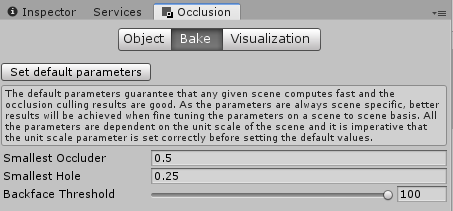
\includegraphics[width=1\textwidth]{./imagenes/cullingdata}
	\caption{Parametros aplicados en la aplicación para el culling}
\end{figure}

\begin{figure}[htb]
	\centering
	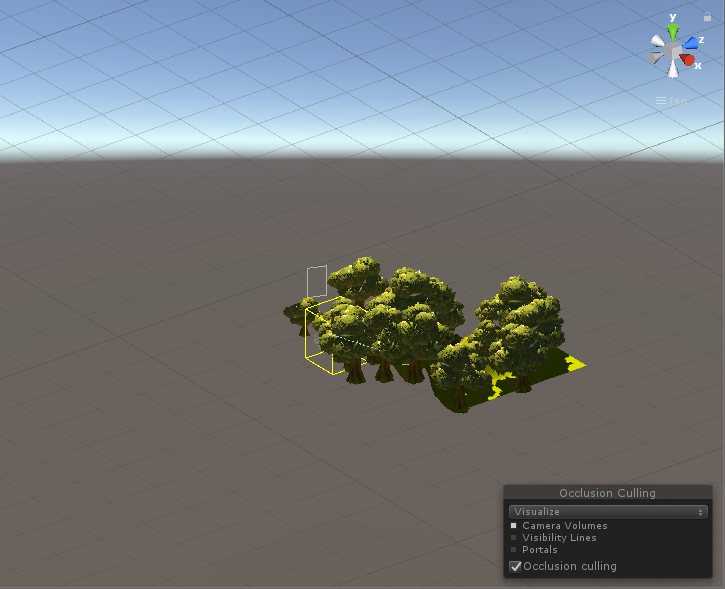
\includegraphics[width=0.40\textwidth]{./imagenes/culling1}
	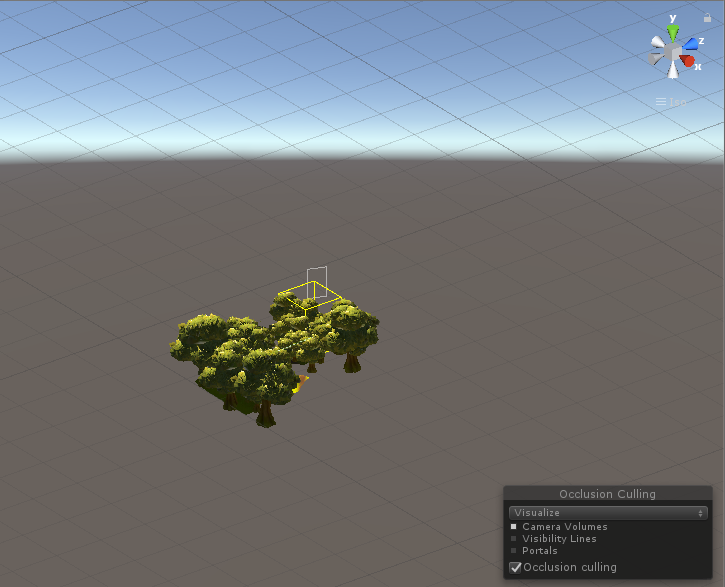
\includegraphics[width=0.40\textwidth]{./imagenes/culling2}
	\caption{Script ResonaceAudioRoom}
\end{figure}

		\subsubsubsection{Pájaros}

\quad El sonido en los pájaros se genera de la misma forma que en cualquier elemento con sonido (el cubo o el icosaedro), aunque presentan una pequeña diferencia. Donde encontremos dentro del script \textit{lb\_Bird.cs} una reproducción de uno de los cuatro audios que componen los sonidos del pájaro, se debe tener en cuenta que ahora el pájaro no contará con un AudioSource propio, si no que ese componente se encontrará dentro del objeto hijo ResonanceAudioSource que se le añadirá.\\

\quad Para poder acceder al componente de este onjeto hijo, se debera cambiar la linea que hace el play por lo siguiente:\\

\lstset{language=[sharp]C, breaklines=true, basicstyle=\footnotesize}
\begin{lstlisting}[frame=single, caption={Ejemplo de cambio de audio para pájaro}]
	this.transform.Find("ResonanceAudioSource").gameObject.GetComponent<AudioSource>().PlayOneShot (song1,1);
\end{lstlisting}

\quad Deben hacerse cuatro cambios en el script \textit{lb\_Bird.cs}.\\

\quad Lo último a tener en cuenta en esta escena, es cambiar el shader de los materiales que componen la escena a \textit{Movile/Diffuse}. De esta forma se garantiza que el shader está optimizado para trabajar en un móvil.\\

\newpage




	\thispagestyle{empty} 
	\textcolor[rgb]{1.00,1.00,1.00}{.} 
	\newpage %inserta un salto de página
	
	%--------------------------------------
	% PRUEBAS
	%--------------------------------------
	
	\section{Pruebas, testeos y fallos}

\subsection{Introducción}

\quad Como es evidente, a lo largo de un desarrollo, por pequeño que sea, aparecen problemas que el desarrollador debe afrontar utilizando sus dotes deductivas y de búsqueda. Dicho esto, es tarea del mismo buscar una solución que arregle el problema encontrado, o una solución alternativa que cambie la forma de enfocar el objetivo.\\

\quad A continuación se presentan un par de casos que aparecieron durante este desarrollo.\\

\subsection{El caso de las retículas rebeldes}

\quad Siguiendo un tutorial de youtube, se intento hacer un temporizador para la interacciones de la retícula con los objetos.\\

\quad El resultado era satisfactorio dentro del entorno en el PC, pero los problemas comenzron al pasar la aplicación al dispositivo móvil, ya que la reticula de carga no se centraba correctamente, provocando una sensación de mareo al no saber sobre que reticula centrarse.\\ 

\quad La solucion por la que se optó al descubrir que todo era producido por un bug interno producido por incompatibilidades entre la versión de Unity y la del paquete GoogleVR no fue igualar versiones, ya que hubiera implicado rehacer practicamente todo el proyecto, si no que se opto por transformar la retícula base y convertirla en un temporizador cuando fuese necesario. Esto implico, como se explica en el apartado \textit{6.5.3. Retícula}, realizar una serie de modificaciones en el shader de google para el material de la retícula.\\

\subsection{La resina del bosque no me permite andar}

\quad La gran carga gráfica del bosque no solo lagueaba la aplicación, si no que además inutilizaba la retícula y el movimiento del personaje, mientras que el movimiento de cámara seguía en funcionamiento.\\

\quad La solución paso por reducir el detalle de los modelados, pero esto no termino de solucionar el problema, por lo que se optó por el culling, asi como cambiar todo los shaders a a los menos pesados con los que contaba Unity.\\

\quad Esta solución ha hecho que el bosque sea jugable por fin, pero si se nota que va un poco más lento que las otras dos escenas, cuya carga poligonal el mucho menor.\\  

\subsection{Biclope involuntario}

\quad Este problema es algo que ocurre a todo los desarrolladores, pero es interesante comentarlo para que quede constancia de que el error humano existe y a veces es necesario descansar y continuar con el trabajo más adelante.\\

\quad El problema que se presentó fue que en algunas escenas, la retícula no interaccionaba con los elementos dispuestos para ello. Esto fue un problema serio en su momento, pues parecía que tocaría rehacer gran parte del trabajo, pero después de un descanso, se percibió que la retícula estaba duplicada en la escena, lo que probocaba que no interaccionara correctamente. Una vez eliminada la sobrante, todo funcionó como la seda.\\

\newpage






	\thispagestyle{empty} 
	\textcolor[rgb]{1.00,1.00,1.00}{.} 
	\newpage %inserta un salto de página
	
	%--------------------------------------
	% ANALISIS DE NEGOCIO
	%--------------------------------------
	
	%\section{Análisis de negocio}

\subsection{Introducción}
 
\subsection{Mercado}


\subsection{Modelo de negocio}


\subsection{Análisis de cliente}

\newpage




	%\thispagestyle{empty} 
	%\textcolor[rgb]{1.00,1.00,1.00}{.} 
	%\newpage %inserta un salto de página
	
	%--------------------------------------
	% CONCLUSIONES Y FUTUROS
	%--------------------------------------
	
	%\section{Conclusiones}

\quad Esta aplicación a resultado apasionate, pues realmente creo que me ha hecho crecer como desarrollador. Digo esto, porque trabajar en un proyecto tuyo, que sabes que quieres hacer y que tu mismo propusiste, puede ser abrumador, pero acaba sacando lo mejor de ti.\\

\quad Por la falta de potencia de procesamiento, tanto del equipo de desarrollo como del movil con el que se iba a trabajar, ubo una idea uqe se tuvo que desechar, que era aplicar Raytracing al concepto de 8D. Esto se va a desarrollar ahora mismo en el apartado siguiente.\\

\subsection{Lineas futuras, Ray tracing}

\subsubsection{Definición y planteamiento para sonido}

\quad El raytracing es un algoritmo para síntesis de imágenes tridimensionales propuesto inicialmente por Turner Whitted en 1980. Está basado en el algoritmo de determinación de superficies visibles de Arthur Appel denominado Ray Casting (1968), en el que se se determinan las superficies visibles en la escena que se quiere sintetizar trazando rayos desde el observador (cámara) hasta la escena a través del plano de la imagen. Se calculan las intersecciones del rayo con los diferentes objetos de la escena y aquella intersección que esté más cerca del observador determina cuál es el objeto visible.\\

\quad En el Raytracing se extiende la idea de trazar los rayos para determinar las superficies visibles con un proceso de sombreado (cálculo de la intensidad del píxel) que tiene en cuenta efectos globales de iluminación como pueden ser reflexiones, refracciones o sombras arrojadas. Para simular los efectos de reflexión y refracción se trazan rayos recursivamente desde el punto de intersección que se está sombreando dependiendo de las características del material del objeto intersecado. Para simular las sombras arrojadas se lanzan rayos desde el punto de intersección hasta las fuentes de luz. Estos rayos se conocen con el nombre de rayos de sombra (shadow rays).\\

\quad Se puede apreciar que en los parrafos anteriores solo se habla de gráficos, lo cuál plantea cómo aplicar esto a sonido. En realidad el concepto es muy similar al lo anterior, se imiten los rayos, pero determinamos las variaciones del sonido por los rebotes en los diferentes elementos en una habitación, determinando el ángulo de entrada más optimo para ese fin.\\

\begin{figure}[htb]
	\centering
	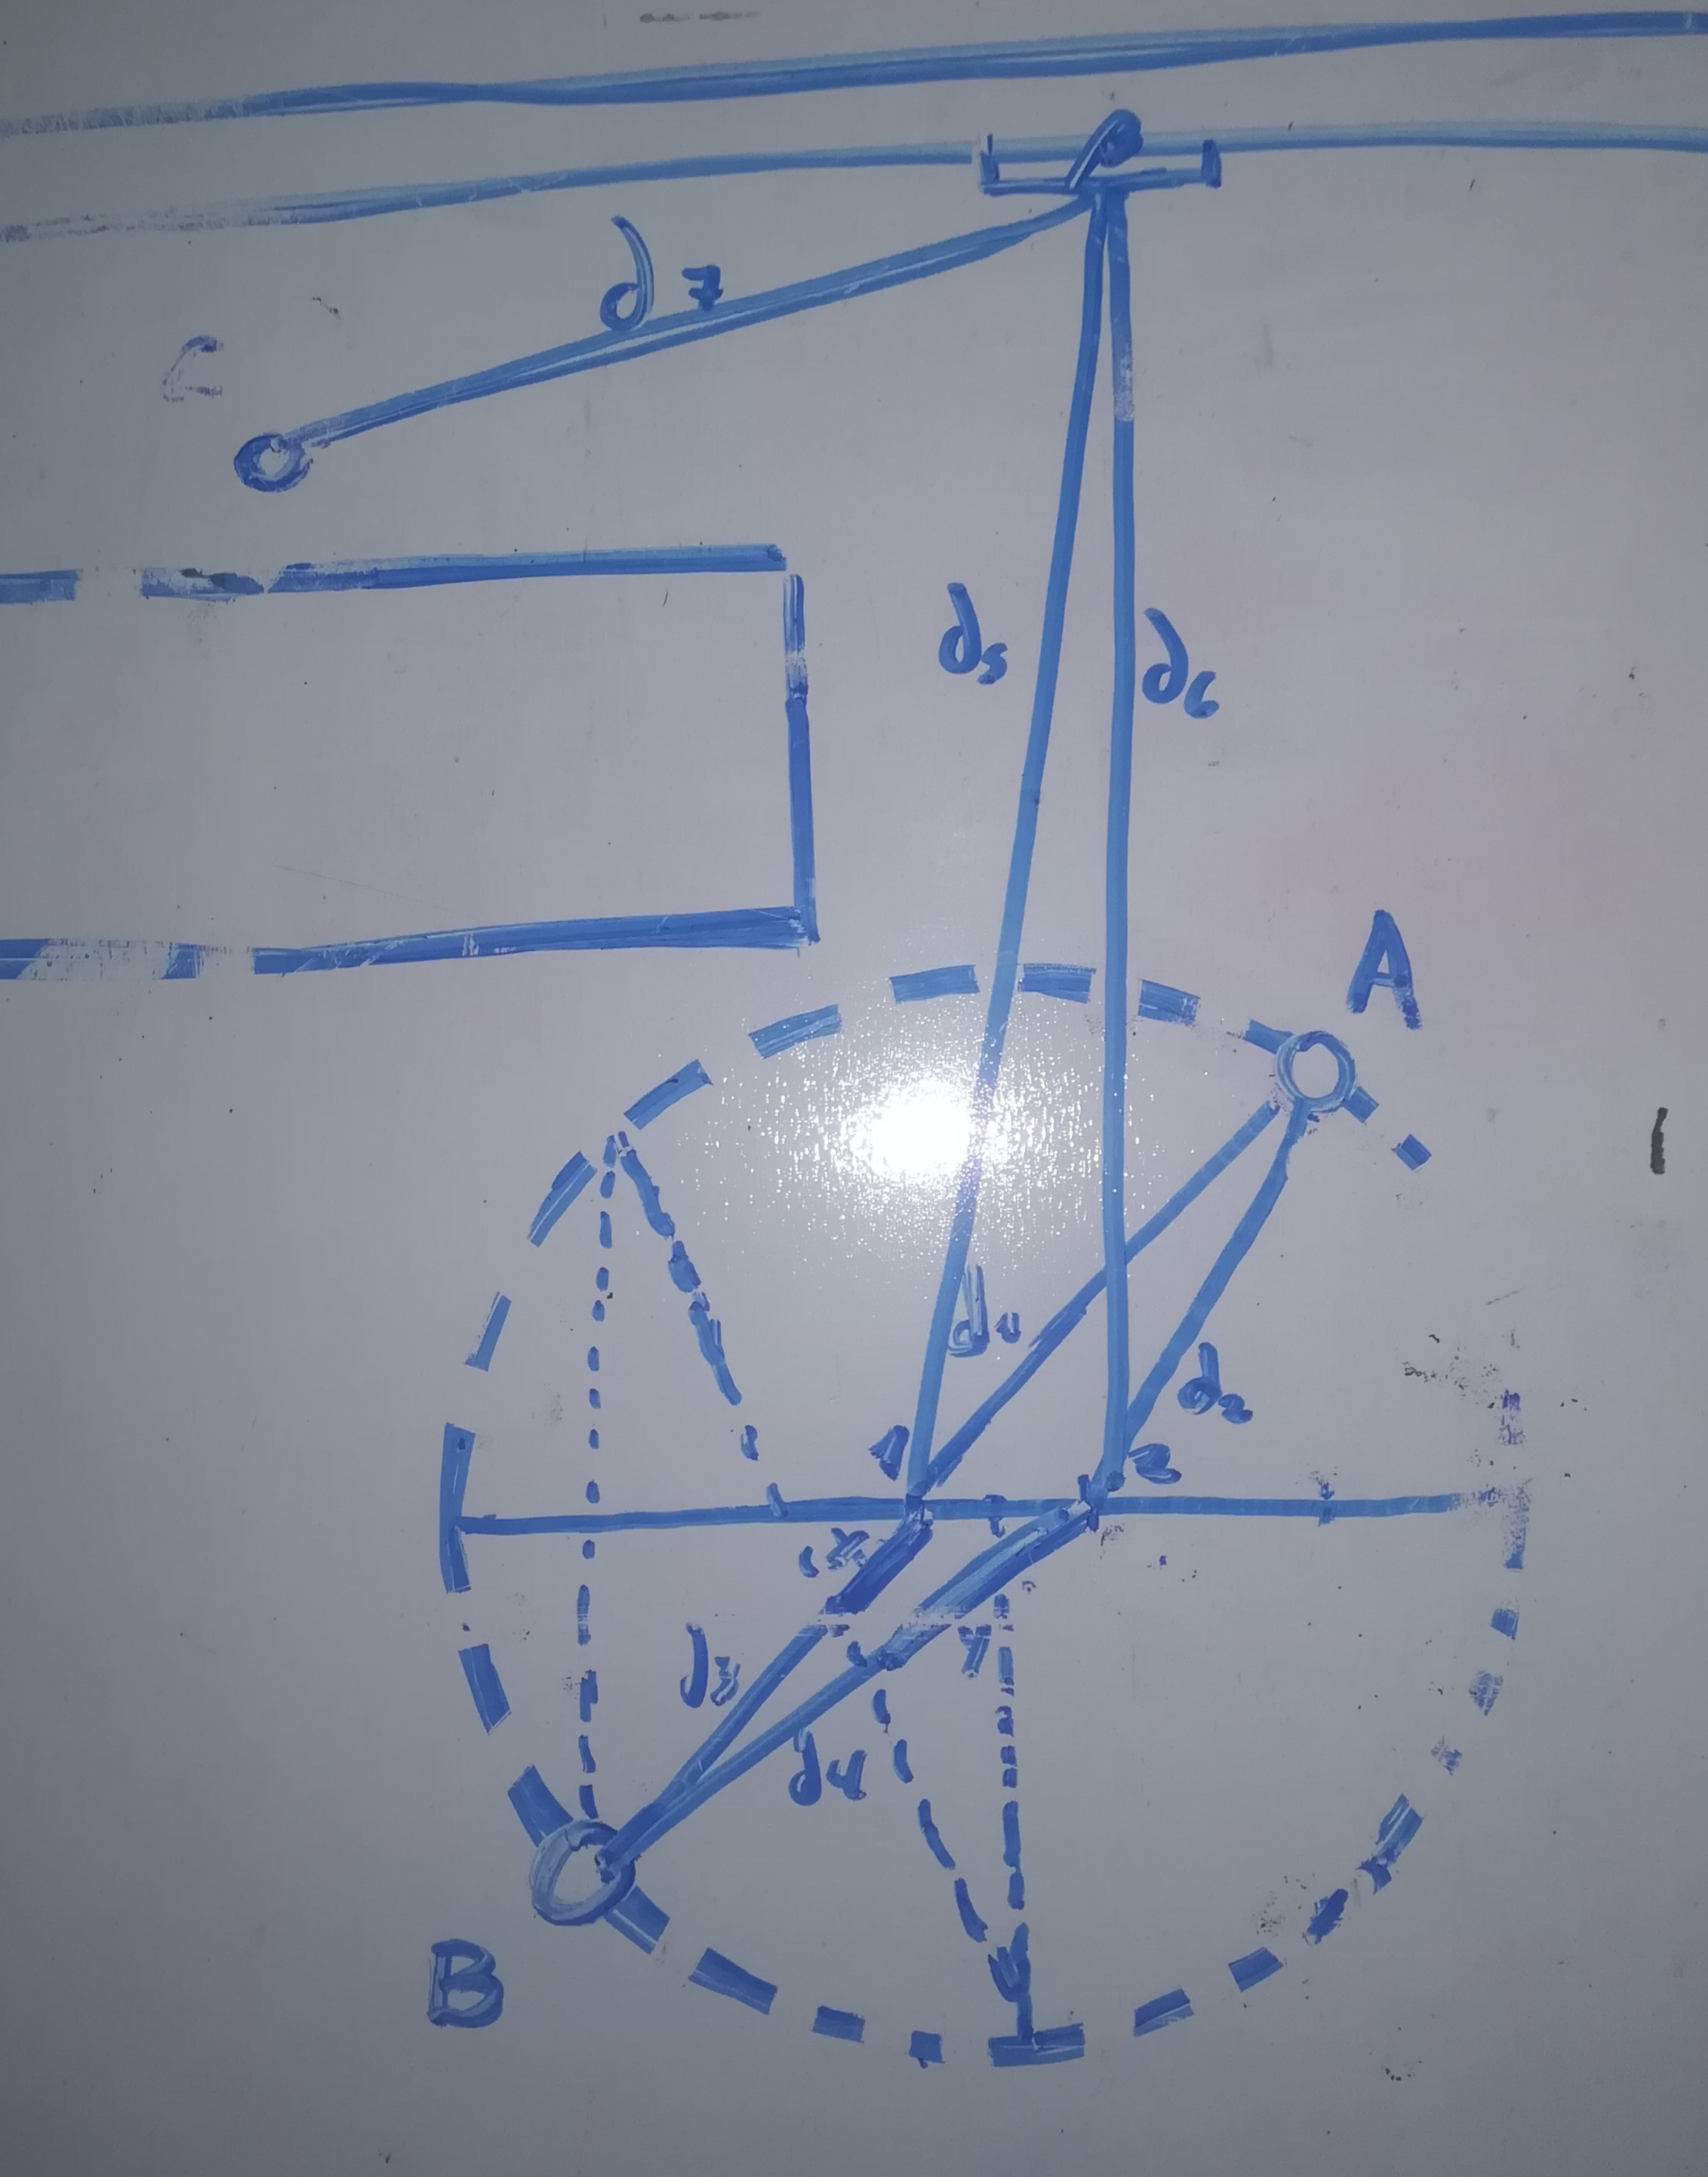
\includegraphics[width=0.5\textwidth]{./imagenes/pizarra}
	\caption{Esquema conceptual en pizarra del raytracing}
\end{figure} 

\quad Gracias a la industria del videojuego, no estamos lejos de poder disfrutar del raytracing de una forma más común, ya que juegos como Cyberpunk 2077 (a día de la redacción de este documento, el juego no ha salido al mercado) plantean el uso de esta tecnología, pero los equipos de los que disponen los jugadores aún no estan a la altura de una carga computacional tan grande. Con todo, solo se puede decir que el cielo es el límite, y que en un futuro no tan lejano, todo lo plateado sobre esta tenología que suena a ciencia ficción, disfrutaremos de todo esto como si fuera lo más común y normal.\\ 

\newpage



	%\thispagestyle{empty} 
	%\textcolor[rgb]{1.00,1.00,1.00}{.} 
	%\newpage %inserta un salto de página
	
	%--------------------------------------
	% MANUAL DE USUARIO
	%--------------------------------------
	
	\section{Manual de Usuario}

\subsection{Primeros pasos}

\quad Lo primero que se debe hacer es disponer de unas cardboard (o similar), asií como de unos auriculares estereo y un móvil con sistema \textit{android 4.4 Kit Kat} para que la aplicación funcione.\\

\quad Teniendo esto en cuenta, la aplicacioón cuenta con tres factores para las interacciones con el entorno: \\

\begin{itemize}
	\item Andar hacia adelante: presionar el botón de la carboard.
	\item Girar la camara: girar sobre uno mismo para que el acelerómetro determine hacia donde miras.
	\item Interaccionar con un elemento: si se puede interaccionar, al apuntar la tetícula hacia el esta cambiará a una barra de carga que, al terminar, desata la interacción asociada.
\end{itemize}

\newpage



	\thispagestyle{empty} 
	\textcolor[rgb]{1.00,1.00,1.00}{.} 
	\newpage %inserta un salto de página
	
	%-----------------------------------------------------------------------
	%							BIBLIOGRAFIA
	%-----------------------------------------------------------------------
	
	\begin{thebibliography}{99}
		\bibitem{Git} 
			\textsc{Tutorial GitFlow}
			\textit{Atlasian}.
			\newline
			\url{https://www.atlassian.com/git/tutorials/comparing-workflows/gitflow-workflow}
		\bibitem{Sha} 
			\textsc{Tutorial shaders}
			\textit{Unity}.
			\newline
			\url{https://docs.unity3d.com/es/current/Manual/Shaders.html}
		\bibitem{Res} 
			\textsc{Librería resonance en unity}
			\textit{Unity}.
			\newline
			\url{https://resonance-audio.github.io/resonance-audio/develop/unity/getting-started}
		\bibitem{Gvr} 
			\textsc{Librería GoogleVR}
			\textit{Unity}.
			\newline
			\url{https://developers.google.com/vr/develop/unity/get-started-android}
		\bibitem{Cul} 
			\textsc{Oclussion Culling}
			\textit{Unity}.
			\newline
			\url{https://docs.unity3d.com/es/current/Manual/OcclusionCulling.html}
		\bibitem{Res} 
			\textsc{Descarga Resonance}
			\textit{Resonance}.
			\newline
			\url{https://github.com/resonance-audio/resonance-audio-unity-sdk/releases}
		\bibitem{Gvr} 
			\textsc{Descarga GoogleVR}
			\textit{GoogleVR}.
			\newline
			\url{https://github.com/googlevr/gvr-unity-sdk/releases}
		\bibitem{Chi} 
			\textsc{Gamificación en China}
			\textit{Gobierno Chino}.
			\newline
			\url{https://innovadores.larazon.es/es/not/gamificacion-de-la-conducta-ciudadana-en-china}	
		\bibitem{8D} 
			\textsc{Sonido 8D}
			\textit{Verdades y mentiras de la nueva forma de escuchar música que te 'hackea' el cerebro}.
			\newline
			\url{https://www.yasss.es/sabiduria-pop/audio-8d-que-es-hackea-cerebro_0_2643900156.html}
		\bibitem{Vre} 
			\textsc{VR en las aulas}
			\textit{La realidad virtual en las aulas: ¿Realidad o virtual?}.
			\newline
			\url{https://www.educaciontrespuntocero.com/noticias/realidad-virtual-aulas-educacion/68851.htmll}	
		\bibitem{Gam} 
			\textsc{Sonido 8D}
			\textit{Verdades y mentiras de la nueva forma de escuchar música que te 'hackea' el cerebro}.
			\newline
			\url{https://www.educativa.com/blog-articulos/gamificacion-el-aprendizaje-divertido/}		
		\bibitem{Csh} 
			\textsc{Gamificación}
			\textit{Gamificación: el aprendizaje divertido}.
			\newline
			\url{https://docs.microsoft.com/es-es/dotnet/csharp/getting-started/introduction-to-the-csharp-language-and-the-net-framework}
		\bibitem{Git} 
			\textsc{GitKraken}
			\textit{Información sobre GitKraken}.
			\newline
			\url{https://support.gitkraken.com}
		\bibitem{Csh} 
			\textsc{Gamificación}
			\textit{Gamificación: el aprendizaje divertido}.
			\newline
			\url{https://docs.microsoft.com/es-es/dotnet/csharp/getting-started/introduction-to-the-csharp-language-and-the-net-framework}
		\bibitem{Git} 
			\textsc{GitKraken}
			\textit{Control de Versiones: ¿Por qué GitKraken?}.
			\newline
			\url{https://medium.com/@sergupe6/control-de-versiones-por-qu%C3%A9-gitkraken-ee1f30b4a18f}
		\bibitem{Cardboard} 
			\textsc{Cardboard}
			\textit{Información sobre las cardboard}.
			\newline
			\url{https://vr.google.com/intl/es_es/cardboard/}
		\bibitem{You} 
			\textsc{Tutorial Retícula}
			\textit{Unity VR Tutorial - Gaze Timer Interaction + Teleport}.
			\newline
			\url{https://www.youtube.com/watch?v=bmMaVTV8UqY}
		\bibitem{Ray} 
			\textsc{Raytracing}
			\textit{Introduction to Ray Tracing: a Simple Method for Creating 3D Images}.
			\newline
			\url{https://www.scratchapixel.com/lessons/3d-basic-rendering/introduction-to-ray-tracing?url=3d-basic-rendering/introduction-to-ray-tracing}


	\end{thebibliography}

	
	% \cite{Baz}
	% \vspace{0.06in}

	%\begin{figure}[htb]
	%	\centering
	%	
\includegraphics[width=0.4\textwidth]{./imagenes/1}
	%	\caption{Universidad de Granada.} \label{fig:1}
	%\end{figure}


	
\end{document}